\documentclass[11pt, a4paper, titlepage]{report}
\usepackage{mathtools}
\usepackage{xcolor}
\usepackage{amsfonts}
\usepackage{minted}
\usepackage{booktabs}
\usepackage[UKenglish]{babel}
\usepackage[en-GB,showdow]{datetime2}
\usepackage{csquotes}
\usepackage{hyperref}
\usepackage{imakeidx} \makeindex
\usepackage[
sorting=none,
hyperref=true,
backend=biber,
style=numeric,
backref=true
]{biblatex}
\addbibresource{references.bib}
\usepackage{pdfpages}
\usepackage{glossaries} \makeglossaries{}
\usepackage{graphicx}
\usepackage{framed}
\usepackage{dsfont}
\usepackage{caption}
\usepackage{parskip}
\usepackage[nameinlink,capitalise]{cleveref}
\usepackage{appendix}
\usepackage{float}
\usepackage{lscape}
\usepackage{multirow}

\graphicspath{ {./img/} }

\newglossaryentry{Word}{ name={word}, description={The smallest
    element uttered in isolation with objective meaning. Not
    necessarily separated by spaces, which is an orthographic
    convention. Different languages have different challenges in
    distinguishing words, where more \textit{synthetic} languages
    convey meaning through changing word inflection, and
    \textit{analytic} languages convey meaning through helper words.
    English straddles the line between these classifications, tending
    more towards analytic than, e.g. German.}}
\newglossaryentry{Term}{ name={term}, description={``a word or
    expression that has a precise meaning in some uses or is peculiar
    to a science, art, profession, or subject''
    \autocite{dictionary:_term_defin_term} --- here text analysts have
    capitalised on the generalisation of ``term'' to include
    subcomponents or aggregations of words} }
\newglossaryentry{Token}{ name={token}, description={A concrete
    instance of a word in text. The phrase ``The cat on the mat'' has
    5 tokens, as the first ``the'' is considered separately to the
    second.}} \newglossaryentry{Text}{ name={text}, description={A
    written communication, in text analytics typically excluding
    ``textuality'' elements such as a reader's interpretation.
    Examples include books, youtube comments, articles, etc.}}
\newglossaryentry{Stem}{ name={stem}, description={The reduced form of
    a created by removing inflections. For example, ``readily'' may
    have the ``ly'' removed to become ``readi''. In linguistic terms,
    the process of morphological (units of meaning) reduction of a
    word.}} \newglossaryentry{Lemma}{ name={lemma}, description={The
    dictionary form of a word. Typically without tense. The lemma of
    ``readily'' is ``ready'', and the lemma of ``is'' is ``be''. In
    linguistic terms, a lemma is the conventional form of a lexeme
    (the basic meaning behind related words).}}
\newglossaryentry{Lexicon}{ name={lexicon}, description={A language's
    inventory of lexemes (lemmas). In text analytics a
    lexicon is typically a dictionary data structure containing a list
    of words and possibly some values for each word.}}
\newglossaryentry{Corpus}{ name={corpus}, description={A collection
    (``body'') of texts, with analysis usually within and between the
    texts.}}
\newglossaryentry{n-grams}{ name={n-gram}, description={A series of
    words that occur in a direct n-length sequence. For example, in
    the phrase, ``The quick brown dog'', the following 2-grams
    (bigrams) exist: ``The quick'', ``quick brown'', ``brown dog''.
    This is generalised to any number of sequential words. They are
    useful in text analytics to determine word sequences, as well as
    common adverb-verb and adjective-noun pairs.}}
  
\begin{document}

% \frontmatter
\begin{titlepage}
  \centering \vspace*{2.5cm}
  {\Huge Enabling Text Analytics}\\
  \vspace{1.5cm}
  {\Large Jason Peter Cairns}\\
  \vspace{1.5cm}
  Supervised by Chris Wild\\
  \vspace{1.5cm}
  \begin{figure}[h]
    \centering 
\includegraphics[height=4cm]{img/uoalogo.png}
  \end{figure}
  \vspace{1cm}
  Bachelor of Science (Honours)\\
  Department of Statistics\\
  The University of Auckland\\
  New Zealand
\end{titlepage}

\thispagestyle{empty} \null{}
\newpage

\begin{abstract}
  Text Analytics serves to reveal insights from a body of text. Within
  the broad category of text analytics, we seek to answer questions
  about what the text is communicating, what is felt about it, and how
  this information is structured. This report describes the creation
  of a user-friendly program to perform text analytics functions,
  using modern \texttt{R} with the Shiny web application framework. A
  literate style illustrates top-down the structure of such a program,
  as well as the data structures and computational processes that have
  established their value for it.
\end{abstract}

\setcounter{page}{1} \pagenumbering{roman}
\chapter*{Acknowledgements}\label{cha:acknowledgements}

I would like to thank my supervisor, Chris Wild, for his constant
encouragement and enthusiasm for the project and my work.

I also thank my family (Bryan, Wendy, Ian, and Caroline) for their
support and understanding during my study.

My thanks also go to those who provided technical advice, especially
Daniel Barnett for advice on Shiny.


% ================================ lists
% ================================

\tableofcontents
\addcontentsline{toc}{chapter}{Listings}
%%%%% \renewcommand\listoflistingscaption{List of Source Codes}
\listoflistings{} \addcontentsline{toc}{chapter}{Tables} \listoftables
\addcontentsline{toc}{chapter}{Figures} \listoffigures

% \mainmatter
\chapter{Introduction}\label{cha:introduction}
\setcounter{page}{1} \pagenumbering{arabic}
\section{Intention}\label{sec:intention}

The intention of this project is to develop a user friendly program
that that allows for the performance of common text analyses. It is
intended to be capable of integrating with iNZight, with a similar
user base. The application is to be flexible enough to deal with a
range of text formats, and produce attractive output quickly. The
application makes a wide range of text analyses easily accessible to
beginners, while still providing significant practical capabilities in
text analytics.
  
\section{Text Analytics Preliminaries}\label{sec:backgr-text-analyt}

Text Analytics is comprised of a variety of processes and techniques
to extract information from text and provide a high-level overview.
The text almost always requires some initial processing. Some of the
following functionalities have proven utility, and are placed in more
context in \underline{\cref{cha:text-analyt-backgr}};

\begin{description}
\item[Sentiment] In order to answer what emotions are conveyed in a
  text, sentiment analysis is commonly performed. The technique yields
  some measure of what is represented in an emotional sense by the
  text, with a range different methods and their associated outputs
  allowing for different forms of the analysis. Sentiment analysis
  won't pick up the subtle nuances that a human reader would, but
  generally gives a reasonable impression over the extent of a text.
\item[Associated Words] The meaning of a text is largely dependent on
  the various structures within and between words. Looking at how
  words are associated, through correlation, common sequences,
  visualisation of sections, etc.,\ allow for high-level investigation
  of the associations between words. The higher level not only saves
  individual efforts, but can demonstrate any emergent properties
  inherent to a text, in a way that a direct reading won't necessarily
  reveal.
\item[Summarisation] Automation of an executive summary, or a list of
  key words, typically falls under the purview of ``summarisation''.
  The primary aim is to rank and select the most ``representative''
  words, combinations of words, or sentences from a text. A few major
  techniques dominate, being somewhat complex in nature. The results
  seem to be surprisingly representative of a text.
\item[Feature Counts] The simplest quantitative measure is very often
  the most informative; from simple word counts, to selective counts
  of sentences within groups, counting features can reveal how much
  written weighting is given to various elements, aiding insight into
  content, structure, and sentiment simultaneously.
\end{description}

\section{Existing Systems}

There are several existing systems in the field of Text Analytics. The
field was initially nurtured as a sub-field of Computer Science, being
computationally-dependent in nature. More recently, there has been
increasing statistical interest. The existing systems reflect this;
most older text analytics programs were Artificial Intelligence
focused, being experimental in nature and typically composed in lisp.
There is also a closely related subfield of linguistics called
``corpus linguistics'', which is served by a small set of R packages
and single-purpose applications performing text analytics
tasks\autocite{desagulier17:_corpus_linguis_statis_r}.

More recently, major statistical programs have been incorporating text
analytic features, with a few smaller text analytics-specific programs
appearing. \texttt{SAS}\autocite{inc.19:_sas_text_miner},
\texttt{SPSS}\autocite{corp.17:_ibm_spss_statis_window_version}, and
\texttt{R}\autocite{team19:_r} are all examples of major statistical processing
systems, with recent additions of text analytics capabilities. An
example of a text analytics-specific application is \texttt{txtminer}, a
commercial web app designed for analysing text at a deep level, with a
linguistic focus, over multiple languages, for an ``educated citizen
researcher''\autocite{bnosac19:_autom_text_analy}. A variety of R
packages aiding in text analytics were assessed and experimented with,
as detailed in \underline{\cref{sec:liter-revi-exist}}.

\section{Background: iNZight}\label{sec:background:-inzight}

iNZight is a statistical analysis suite developed at the University of
Auckland\autocite{wild:_data_analy}. It provides rapid analysis and
visualisation of data in a user-friendly format. It is used by data
journalists, students, and researchers, among others.

Our program will form part of the suite of modules extending iNZight.
It provides a simple GUI interface to rapidly perform common text
analyses. The primary audience for this text module are those learning
the fundamentals and potential of text analysis, which could include
students of the traditional text analytics fields of Statistics and
Computer Science, but can and should include students of Linguistics,
Communications, Law, History, and any other text-based field. Beyond
the educational aspects of the program, it is fully functional for
practical use for general text analysis. Of particular interest in
applied statistics is the exploration of data from free-response items
in surveys.

\section{Literature Review}\label{sec:liter-revi-exist}

The initial review of existing literature was informed by the scope
desired for the program, with \texttt{R}-related sources forming the bulk of
the literature.

Two textbooks were read to begin with, both being related to R:\
``\textit{Text mining with R:~A tidy approach}''\autocite{silge2017text}, and
``\textit{An Introduction to Text Processing and Analysis with
R}''\autocite{clark2019text}. \textit{Text Mining with R} was the
prompt to use a ``tidy'' approach to text analytics, which has proved
to be useful in interactive analysis, though inappropriate for
development (discussed further in \underline{\cref{sec:why-tidyverse}}).

The Natural Language Processing (NLP) task view on CRAN maintains
references to high quality packages relating to text
analytics\autocite{wild:_cran_task_view}. The following packages were
consulted and experimented with:

\begin{description}
\item[\texttt{tidytext}\autocite{Silge2016tidytext}] is a text-mining
  package using tidy principles, providing excellent interactivity
  with the tidyverse, as documented in the book \textit{Text mining
    with R:~A tidy approach}\autocite{silge2017text}.
\item[\texttt{tm}\autocite{feinerer18}] is a text-mining framework
  that was the main package for text mining in \texttt{R}, but appears
  to have been made redundant by \texttt{tidytext} and
  \texttt{quanteda} of late.
\item[\texttt{quanteda}\autocite{benoit18}] sits alone next to
  \texttt{qdap} in the Pragmatics section of the NLP task view, and
  offers a similar capability to \texttt{tidytext}, though from a more
  object-oriented paradigm, revolving around ``corpus'' objects. It
  also has extensions such as offering readability scores, something
  that may be worth implementing in the future.
\item[\texttt{qdap}\autocite{rinker19qdap}] is a ``quantitative discourse
  analysis package'', with an extremely rich set of tools for the
  analysis of discourse in text, which may arise from plays, scripts,
  interviews etc. It includes output on length of discourse for
  conversational agents, turn-taking, and sentiment within passages of
  speech.
\item[\texttt{sentimentr}\autocite{rinker19sent}] is a rich sentiment analysis
  and tokenising package, with features including handling negation,
  amplification, etc.\ in multi-sentence level analysis. An
  interesting feature is the ability to output text with sentences
  highlighted according to their inferred sentiment.
\item[\texttt{dygraphs}\autocite{vanderkam18}] is a time-series visualisation
  package capable of outputting very clear interactive time-series
  graphics, useful for any time-series in the text analysis module.
\item[\texttt{gganimate}\autocite{pedersen19}] produces animations on top of
  the \texttt{ggplot2} package.
\item[\texttt{textrank}\autocite{wijffels19}] implements the
  ``TextRank'' algorithm to extract keywords automatically from a
  text.
\item[\texttt{ggpage}\autocite{hvitfeldt19ggpage}] produces impressive
  page-view charts with word highlighting, allowing for a clear
  overview of a text and it's structure.
\item[\texttt{udpipe}\autocite{wijffels19:udpipe}] performs tokenisation, parts
  of speech tagging (which aids textrank), and more, based on the
  well-recognised \texttt{C++ udpipe}, using the ``Universal Treebank''.
\item[\texttt{BTM}\autocite{wijffels19:_btm}] performs ``Biterm Topic
  Modelling'', which is useful for ``finding topics in short texts (as
  occurs in short survey answers or twitter data)''. It uses a
  somewhat complex sampling procedure, and like LDA topic modelling,
  requires a corpus for comparison. The \texttt{BTM} \texttt{R}
  package is based on the \texttt{C++ BTM}.
\item[\texttt{crfsuite}\autocite{wijffels18crf}] provides a complete modelling
  framework, which is outside our scope, but could be useful later.
\item[\texttt{humaniformat}\autocite{keyes16}] is useful in the analysis or
  removal of personal names, by providing a dictionary and properties
  of thousands of names.
\item Packages for obtaining text:
  \begin{description}
  \item[\texttt{gutenbergr}\autocite{robinson19}] can search and
    download texts from \textit{Project Gutenberg} directly.
    \textit{Project Gutenberg} is the largest public online repository
    of public domain books.
  \item[\texttt{rtweet}\autocite{rtweet-package}] can directly attain tweets
    from the social media site \textit{twitter}. It requires an API key from
    \textit{twitter}, which is an arduous process to obtain.
  \item[\texttt{WikipediaR}\autocite{bar-hen16:_wikip}] can download \textit{Wikipedia}
    pages and associated metadata directly.
  \end{description}
\end{description}

\section{Scope of work}\label{sec:scope-work}

The total scope possible for text analytics is near endless. As such,
it is essential that limits were placed the scope of this program.
There are two primary areas of limitation: text type, and analysis type.

By limiting the forms of text worked with, less effort was required to
be spent on consideration of every single possible import and
transformation case, and more time on the actual design of analysis.
The simplest means with which to create the limitation exists in
allowing only import of particular text-file formats --- in this case,
import caters only for flat \texttt{txt} files, as well as tabular
\texttt{csv} and \texttt{xlsx} files. What is not provided is access
in-program to common text sources through their API, such as Twitter
or Project Gutenberg.

Through focusing on dictionary-based, rather than model-based
analyses, we have avoided much of the associated complexities of
modelling. An example of this is that it is common to categorise words
based on their grammatical category, then use models that take the
categories into account. By avoiding that, there has been far more
functionality implemented in a shorter amount of time, with the
analyses still performing soundly. Additionally, the primary focus is
on a general audience, and it is typically only more advanced,
linguistically-trained users who would make intelligent use of very
complex analyses.

\chapter{Text Analytics Background}\label{cha:text-analyt-backgr}

Text analytics is often considered a sub-field of data science, which
is the extraction of insight from structured and unstructured
data\autocite{rajman1998text}.

Text analytics is less commonly associated with statistics proper,
given that much of the methodology is computer science heavy. The
program developed in this project encourages a statistically-based
analysis for text, giving emphasis to summary statistics of analyses,
as well as distributions of results.

Many text analytics analytics solutions are in fact computer science
based, rather than statistical. In this sense, text analytics mirrors
data science closely, with much of the development occurring in
computer science departments, and some breakthrough models introduced
by statisticians. For example, the ``bag of words'' model was expounded
upon by computer scientists (in association with linguists), along
with most other models, to the point where ``text mining'', the name
more commonly associated with text analytics in the past, was
effectively treated as a sub-field of computer
science\autocite{ko2012study}. However, many important models are very
statistical in nature, such as Latent Dirichlet allocation, which uses
complex Bayesian inference, and was developed in conjunction with
statisticians\autocite{blei2003latent}.

\section{Overview}\label{sec:overview}

Having as it's object of interest textual communication, text
analytics borrows much of the vocabulary of linguistics. Some
important concepts allow us to speak the language of text analytics:

\begin{description}
\item[\gls{Word}] The smallest element uttered in isolation with
  objective meaning. Not necessarily separated by spaces, which is an
  orthographic convention.
\item[\gls{Term}] ``a word or expression that has a precise meaning in
  some uses or is peculiar to a science, art, profession, or subject''
  \autocite{dictionary:_term_defin_term} --- here text analysts have
  capitalised on the generalisation of ``term'' to include
  sub-components or aggregations of words.
\item[\gls{Token}] A concrete instance of a word in text. The phrase
  ``The cat on the mat'' has 5 tokens, as the first ``the'' is
  considered separately to the second.
\item[\gls{Text}] A written communication, in text analytics typically
  excluding ``textuality'' elements such as a reader's interpretation.
  Examples include books, YouTube comments, articles, etc.
\item[\gls{Stem}] The reduced form of a word, created by removing
  inflections. For example, ``readily'' may have the ``ly'' removed to
  become ``readi''; in linguistic terms, the process of morphological
  (units of meaning) reduction of a word.
\item[\gls{Lemma}] The dictionary form of a word. Typically without
  tense. The lemma of ``readily'' is ``ready'', and the lemma of
  ``is'' is ``be''. In linguistic terms, a lemma is the conventional
  form of a lexeme (the basic meaning behind related words).
\item[\gls{Lexicon}] A language's inventory of lexemes (lemmas). In
  text analytics a lexicon is typically a dictionary data structure
  containing a list of words and possibly some values for each word.
\item[\gls{Corpus}] A collection (``body'') of texts, with analysis
  usually within and between the texts.
\end{description}

\section{Terms}

At the centre of text analytics are words. Different models of text
analytics typically differ over the basis by which they treat words.
For example, the ``bag of words'' model only considers the list of
unique words in a document, and how many each of these occur. The
framework used in this project is based on the ``tidy approach'',
wherein each word is considered a distinct element of a vector, which
may, as a whole, represent a text. This can be aligned with other
information, in the form of a data frame. The tidy approach preserves
ordering, unlike the bag of words model.

A significant benefit of maintaining the ordering of the words of a
document is that structural information is preserved, allowing for
analysis of the emergent structures within a text. If additional
information on sentences, chapters, or other textual groupings are
preserved or inferred (and this program is capable of both), then
these structures can be analysed in their own right. Common structures
include sentences, chapters, documents, and n-grams:

\begin{itemize}
\item[\gls{n-grams}] A series of words that occur in a direct n-length
  sequence. For example, in the phrase, ``The quick brown dog'', the
  following 2-grams (bi-grams) exist: ``The quick'', ``quick brown'',
  ``brown dog''. This is generalised to any number of sequential
  words. They are useful in text analytics to determine word
  sequences, as well as common adverb-verb and adjective-noun pairs.
\end{itemize}

\section{Framework}\label{sec:framework-used}

Text analytics follows much of the same process
(\underline{\cref{fig:std-ds}}) as many other data science analyses.
We have identified three main sections of a standard text analysis,
being processing, ``insights'', and visualisation. ``Insight'' here is
a word we have specialised the meaning of to capture the concept of
producing statistical summaries or sets of summaries from processed
text. The three sections identified are similar to the data science
process, however due to the lack of structure present in most text
data formats, extra processing is typically required to infer or
associate structure. The various processes of attaining insight
typically follow a similar functional process with a standard input
and standard output, with some notable exceptions. Visualisation is
often similar to other statistical analyses, though the nature of text
presents some unique challenges and opportunities

\begin{figure}[h]
  \centering 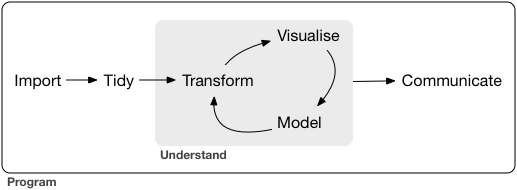
\includegraphics[scale=0.8]{std-ds.png}
  \caption{Standard data science
    process\autocite{wickham2016r}\label{fig:std-ds}}
\end{figure}

\subsection{Processing}\label{sec:processing}

Processing is the first component of every text analysis, commonly
returned to and modified within an analysis. Processing refers to the
import, cleaning and transformation of text data. It is performed in
order to attain a standard structure for text data, which is
notoriously unstructured. The data is generally very messy, requiring
significant effort to clean and ``tidy''.

Importation of text data is fairly simple, being no different to the
import of any other data. However, words need to be separated, a
process known as ``tokenisation''. Once words are separated and kept
separate through some data structure, words that are unnecessary for
analysis are removed. Text analytics is opposite to most statistical
analyses in this respect; unusual data points may sometimes be removed
in statistical analyses as outliers, but common words that render no
insight, such as articles like ``the'', are commonly removed in a text
analysis. These removed words are known as ``stopwords''. The
remaining words may be transformed into lemmas or stemmed. As text
files often have no metadata indicating internal structure such as
chapters, these can be inferred through a process created by this
project, which we call ``sectioning''. Finally, the processed data is
pulled together into some standard data structure, and fed through to
the next part of the text analytics process.

\subsection{Insight}\label{sec:insight-1}

After the text data has been made malleable enough through processing,
it is ready for analysis to produce some ``insight measure'', wherein
various statistics and scores can be computed from the processed text.

In order to attain useful information about the text, ``insight''
functions can be applied to the data, giving metrics relating to
various properties of the text which can capture important information
about the text.

Most of our insight functions will compute some score or statistic for
texts. These may be applied at the individual word level, or at some
aggregate level. Key functions include the frequency count of words,
n-grams and n-gram frequency, summary scores, and correlations between
words. Sentiment is a common score that is computed to map the
emotional charge of a particular word to some numeric score, or
emotional category. The program implements all of these functions, as
well as some unique and experimental variations on them. Other common
analyses include determining the frequency of words in several
individual documents relative to their overall frequency, known as
``term frequency --- inverse document frequency'', and inferring
common topics in a text, known as ``topic modelling''

\subsection{Visualisation}\label{sec:visualisation-1}

A clear way to display and communicate the result of an analysis or
exploration is through visualisation. Visualisations are applied to
``insights''. Typically a variety of different visualisations are
available to be applied any particular insight measure.

When visualising text, most insight measures produce a numeric output.
These numeric scores or statistics can be visualised through common
statistical graphics, such as bar plots, histograms, density plots,
etc. When each word of text is considered a step forward through time
in a text, the scores of each word may be used to plot a time series.
Uniquely to the visualisation of text, the property belonging to each
word or group of words can also be visualised as an overlay on the
original page of text --- known as a ``page view''. The words
themselves may be used as the central piece of a visualisation beyond
the bounds of a page, with ``word clouds'' sizing words according to
their insight score, and laying them randomly about a plot.

Alternative visualisations were explored, with much experimentation
regarding different displays of sentiment insights through
scatterplots. However, these were found to be difficult to interpret.
The only visualisations maintained are those satisfying the
constraints of clarity and ease of interpretation.

\chapter{Program Structure \&
  Development}\label{cha:program-structure}

\section{Preliminaries}\label{sec:preliminaries}

The structure and development of the program has been based mainly on
compatibility with the existing system of iNZight Lite. The current
form of iNZight Lite uses \texttt{R} to perform analyses and handle
data, with the interface using Shiny, an \texttt{R} package allowing
for declarative UI and server definitions to compose a web app, in a
framework similar to JavaScript's react.js\autocite{chang19}. Much of
the program has been written in a functional form, which is idiomatic
of R. This has extended to make use of a constellation of packages
known as the ``Tidyverse''\autocite{wickham17tidy}, including
``ggplot2''\autocite{wickham16ggplt}, for graphic visualisations. This
text analytics program followed that lead, using both \texttt{R} and
Shiny, as well as the functional paradigm with the tidyverse.

\subsection{Why R?}

Aside from compatibility, \texttt{R} is a language well suited to text
analytics in it's own right, with the vectorised semantics mapping
well to the problem space of long sections of text. The package
ecosystem is also very well equipped to handle text analytics, with
the official package repository, CRAN, being audited to maintain a
high level of quality that other repositories such as npm or pip,
don't come close to achieving.

\subsection{Why Shiny?}

Shiny is the default choice for creating web-friendly interfaces in R.
Funded and developed by RStudio, it is typically made use of for
dashboard creation, though it has even been put to use as a chat
client. Shiny makes use of the react style of interface and server
declaration, in which state is heavily de-emphasised in the semantics
of the code, thus keeping the paradigm as declarative as reasonably
possible for a dynamic application. This has some drawbacks, where
state may be useful if an object is to have transformations
iteratively performed on it.

\subsection{Why Tidyverse?}\label{sec:why-tidyverse}

The Tidyverse is ``an opinionated collection of packages designed for
data science'', which is primarily used in this project for data
manipulation with the included package
``dplyr''\autocite{wickham19dpl}, and visualisation with ``ggplot2''.
The packages in the collection have mostly consistent syntax and
style, and are built around the underlying principle of ``tidy data'',
wherein the central working object is a dataframe or dataframe
derivative, with a ``long'' format, where every column is a variable,
and every row is an observation\autocite{wickham2014tidy}. This allows
for great consistency and ease of manipulation, as there is only one
datatype to manage. My text analytics package was designed with this
philosophy in mind, maintaining tidy data and using tidyverse
functionality at all times, which has greatly aided in consistency and
standardisation of development.

However, not all data is modelled well by a tidy dataframe, especially
the hierarchical data inherent in much of text analytics. In these
cases, adherence to tidyverse principles has become more of a
hindrance than a help. The over-emphasis on the tibble (dataframe)
class, encouraged by the tidyverse, has been an unnecessary constraint
for development. All of the more recent functionality in the program
has made decreasing use of the tidyverse aside from ggplot2, which has
the unparalleled ability to facet plots easily based on some grouping
variable --- demonstrated in our application through
\underline{\cref{fig:visualisation-facetting}}.

The use of non-standard evaluation is also set up to work well for
interactive data analysis, though for development purposes, the need
for quoting and unquoting symbols and names has led to a large amount
of unnecessary overhead relative to simply using string-based
selection.

\begin{figure}
  \centering 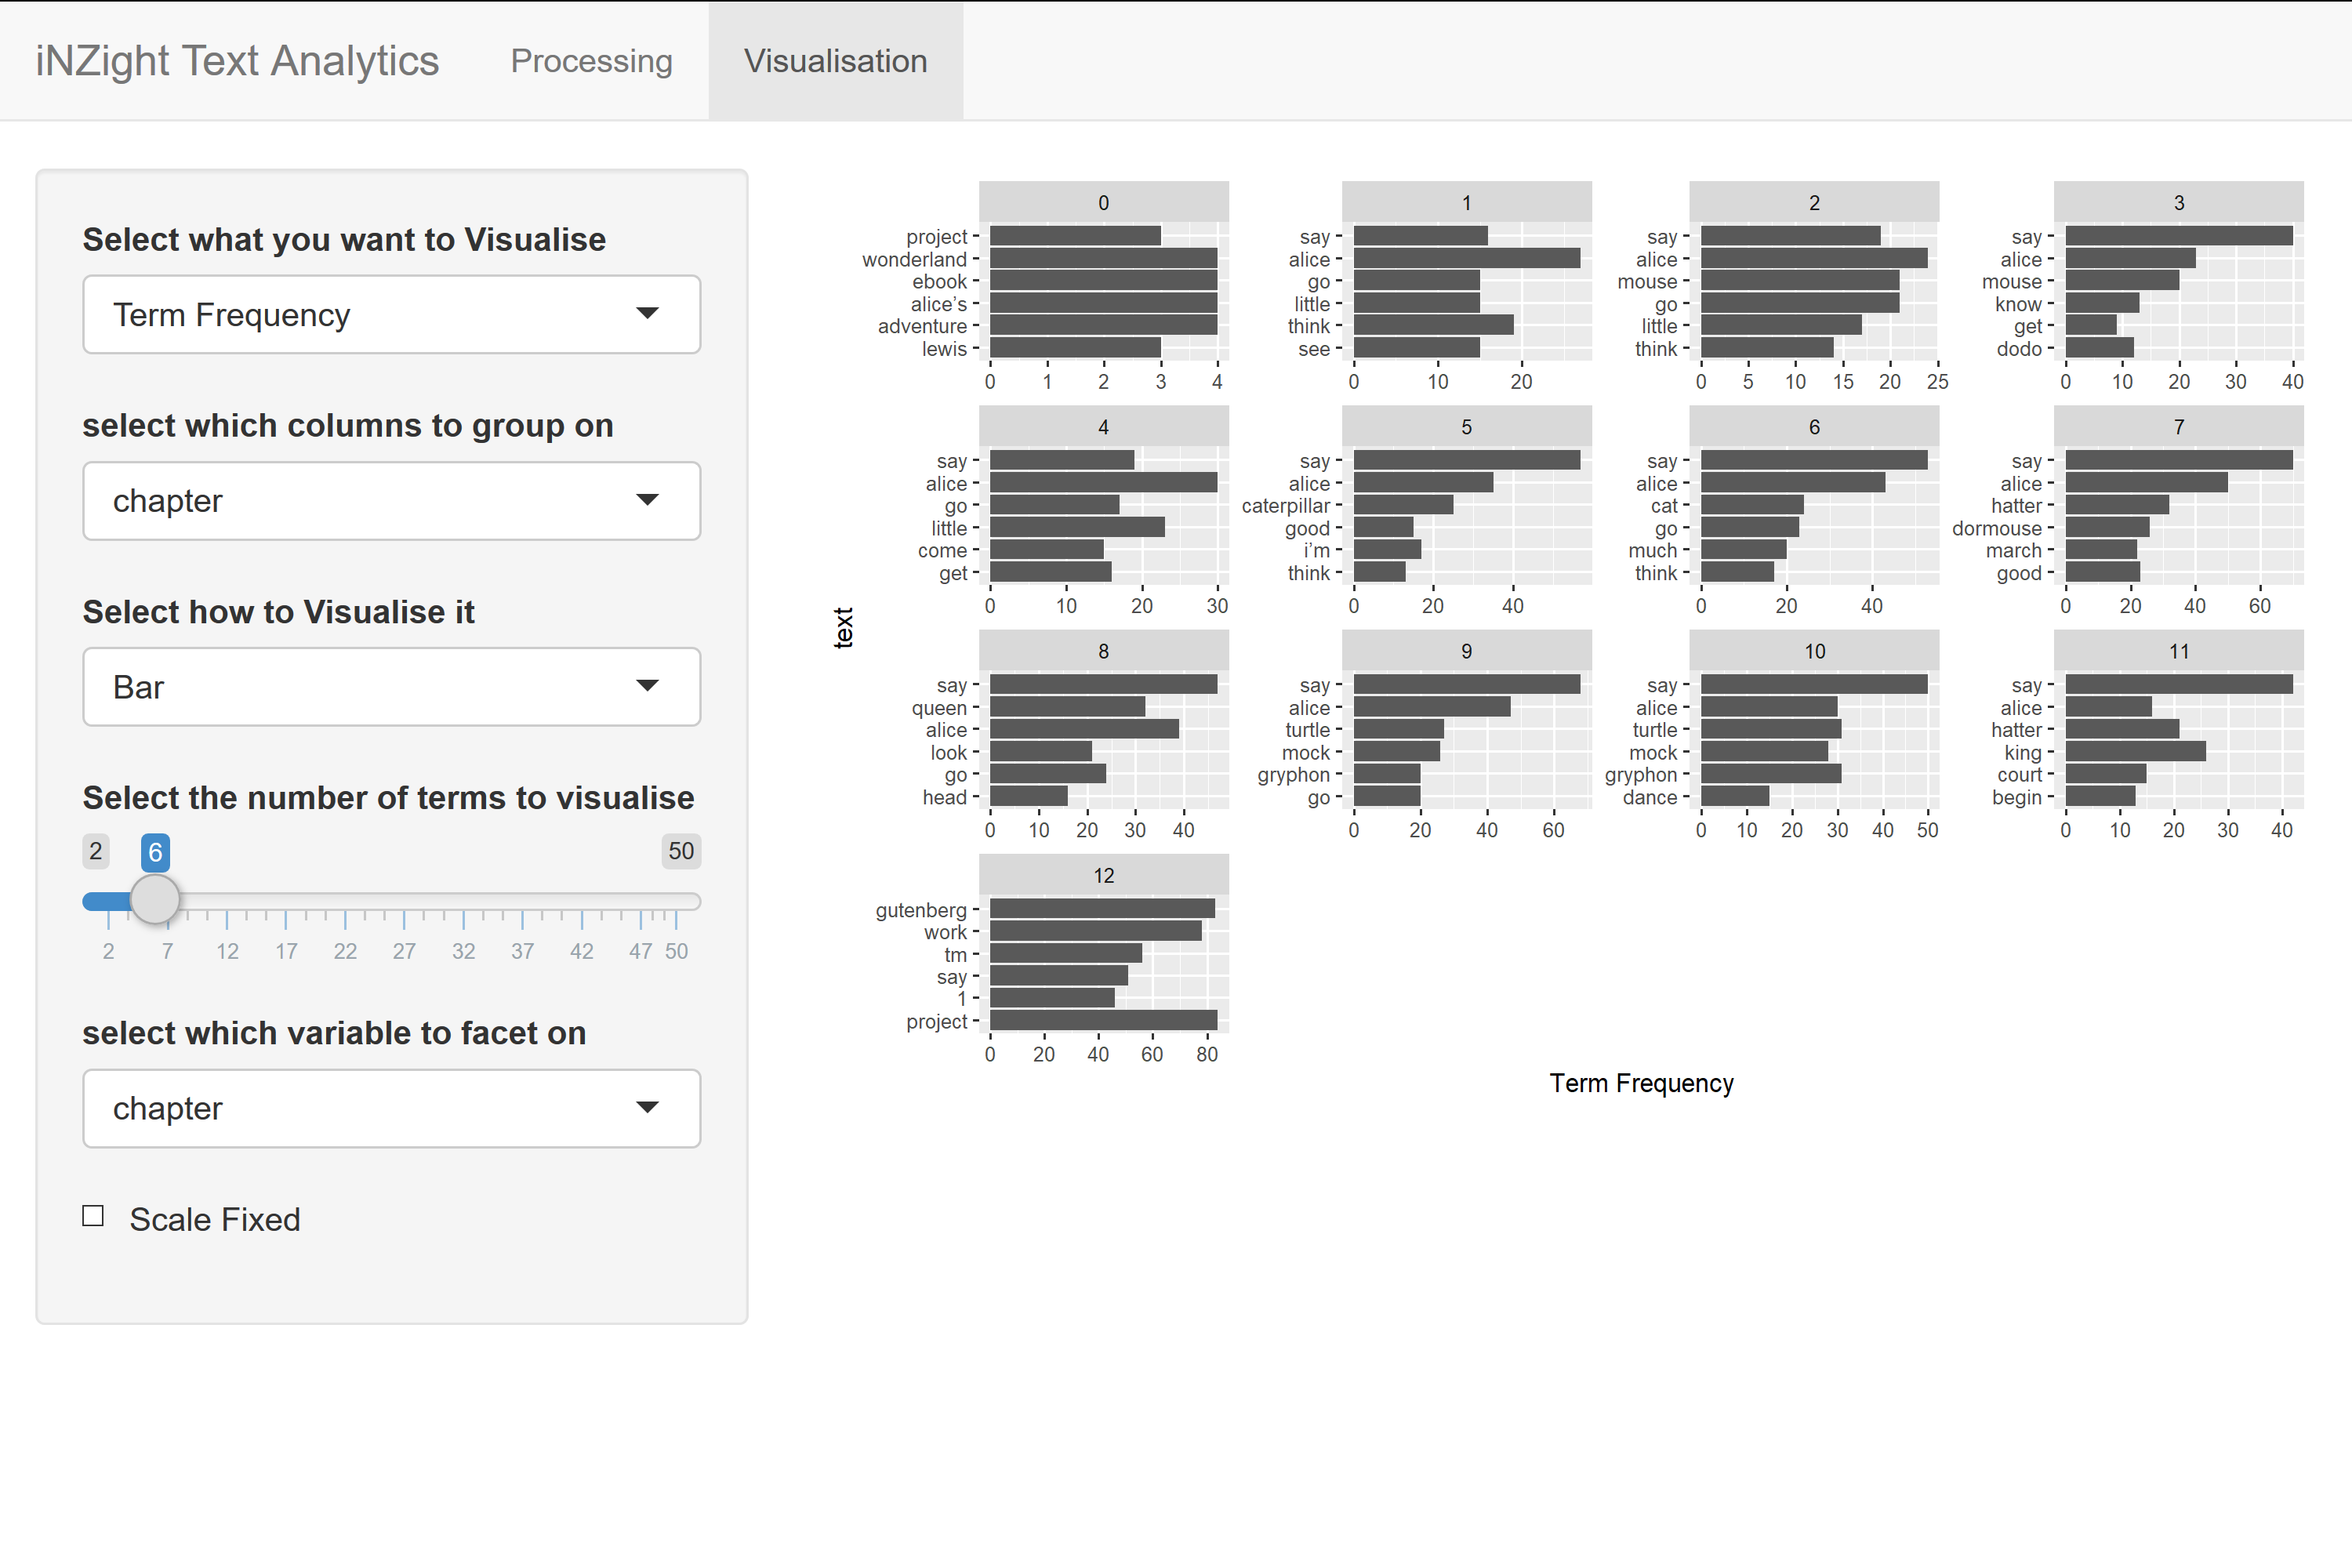
\includegraphics[scale=0.35]{visualisation-facetting.png}
  \caption{Visualisation of
    facetting\label{fig:visualisation-facetting}}
\end{figure}

\subsection{Why Functional?}\label{sec:why-functional}

Functional Programming is a programming paradigm placing emphasis on
pure functions, with no state in the program. Every function has a
surjective mapping from input to output, so for the same input, no
matter what else has happened in the program, the same output should
be expected. This is often contrasted with object-oriented
programming, wherein objects are created that change state as the
program progresses. Assignment of the form, \mintinline{r}{x <- x +
  1}, would not exist in a functional program, as the same variable
\mintinline{r}{x} changes reference at different points. Thus, for-
and while- loops are typically lacking, as they depend on mutating
variables with each iteration. The text analytics program is nearly
entirely functional, with the exception of simple I/O, and some
functions that would be obfuscated in meaning if made functional, such
as \mintinline{r}{get_ngram()}. Functional programming has brought
benefits of easy debugging, as state is no longer a consideration, and
an ability to reason about functions in mathematical terms.

\subsection{Why lossless data?}

The largest issue with keeping the program functional
(\underline{\cref{sec:why-functional}}) and tidy
(\cref{sec:why-tidyverse}) has been the issue of maintaining the
history of the text data. Because there is no state, history can be
difficult to maintain in a memory-efficient manner, and for
transformations on text, history is essential to have at hand. A
notable example is the issue of stopword removal; if stopwords are
removed, with nothing indicating their original location, and the
subsequent text is plotted as a page view, the actual structure of the
original text is missing, with no means to indicate where stopwords
are. Thus the central data structure had to be designed to be as
lossless as possible. This was achieved in the form of a dataframe,
with a column keeping the original text, and a new column holding the
text to be analysed, equivalent to the original text column, but
possibly transformed with lemmatisation, and stopwords ``removed'' by
replacing them with \mintinline{r}{NA} values. Every row corresponds
to a single word from the original text, thus the data structure is
congruent with tidyverse functions.

\subsection{Why Git?}

Git was used from start to finish of development for version control.
Git was used instead of other version control systems such as
subversion or mercurial due to the networking effect, as collaboration
is made easier with all being familiar with the use of GitHub as a
centralised repository. In addition, the \texttt{R} ``remotes''
package and Shiny itself allow for the direct download and
installation of the entirety of the text analytics package and web
application, as in \underline{\cref{lst:inst-shiny}}.

\begin{listing}[ht]
\begin{minted}[frame=lines,fontsize=\scriptsize,xleftmargin=\parindent,linenos]{r}
install.packages(c("remotes", "shiny"))
remotes::install_gitlab("jasoncairns/inzightta")
shiny::runGitHub("jcai849/inzightta-shiny")
\end{minted}
\caption{Installation of package and prototypical deployment of app\label{lst:inst-shiny}}
\end{listing}

\section{Program Architecture}\label{sec:program-architecture-1}

The program is composed of an \texttt{R} text analytics package,
developed over the course of this project, and a web application,
developed towards the end. The package is composed of three separate
sections, being Preparation, Insight, and Visualisation. This serves
to provide functionality from the start to the finish of a text
analysis. The web application is composed of a UI (user interface) and
a server, reliant on the package. The interface is largely generated
server-side depending on the form of the analysis. The server does
much of the coordination for the application, sending options
specified by the user in the UI over to the functions defined in the
package, and returning the results, acting much like the
``controller'' in the model-view-controller framework of software
engineering. A diagram of the program as a system is shown in
\underline{\cref{fig:pr-arch}}.

\begin{figure}
  \centering 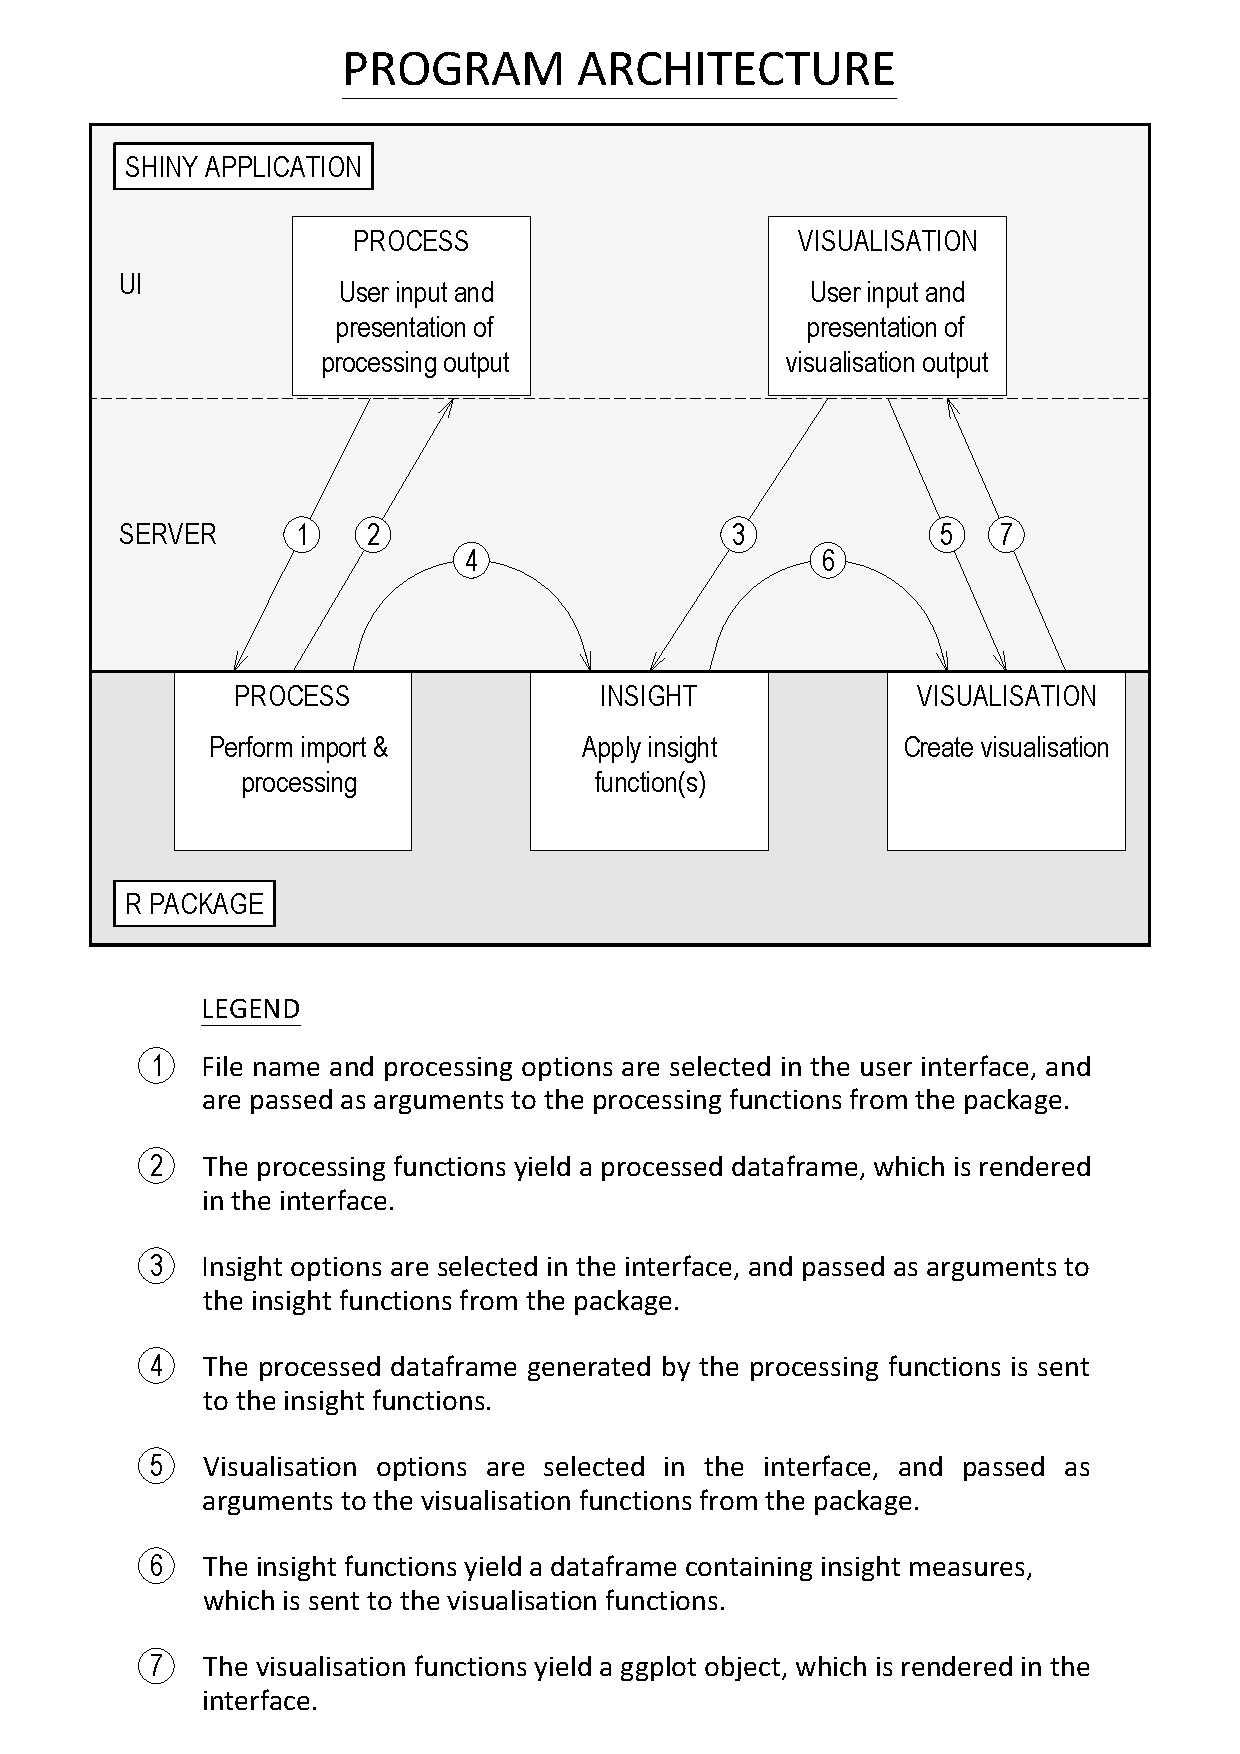
\includegraphics[scale=0.65]{arch-expanded.pdf}
  \caption{Program architecture\label{fig:pr-arch}}
\end{figure}

The program has been structured in this manner to make it as modular
as possible, to the point where, with some minor further development
on the package, it could be released on CRAN as a powerful text
analytics \texttt{R} package in it's own right.

\subsection{Package Description and Creation}

The package, given the working title ``iNZightTA'' (iNZight Text
Analytics), serves to provide all of the background functionality for
the program. In all, there are over 50 major functions defined, as
well as numerous utility and anonymous functions.

Package development mostly followed a ``best practices'' procedure,
with file structure following standard \texttt{R} patterns. The
documentation made use of \texttt{Roxygen2}\autocite{wickham18roxy},
and a 30 page manual was automatically generated from inline function
comment documentation. Testing was performed on a variety of text
types, including free-form survey responses in the form of
\texttt{csv}'s, and novels from \textit{Project Gutenberg} in the form of
\texttt{txt} files.

Dependencies are a necessary evil, and care was taken to include only
highly regarded packages. The \texttt{tidytext} package was made
extensive use of due to it's advocacy by the author of the textbook,
\textit{Text mining with R} (who is also the author of the
package). Unfortunately, despite the online acclaim for
\texttt{tidytext}, the author's poor development practices lead to
several updates of the \texttt{tidytext} package having backwards
incompatible changes, including functions outputting a completely
separate class of object to what was output previously, and the
documentation not being updated to reflect these changes. Upon deeper
inspection of the package source code, investigating several issues,
it was found that most of the functions are wrappers around equivalent
functions provided by other packages. This has created a consistent
interface, but on measure, has not provided enough of a benefit to
justify the issues encountered via the very leaky abstraction.

\section{Preparation}\label{sec:import}

The first step in all text analysis is to import the text data and
wrangle it into a data structure suitable for statistical analysis. In
this case, the data structure for all filetypes is designed to be
lossless, in the form of a dataframe that retains the original text.
This was a key design decision, to avoid ``destructive edits'', which is
the practice where the original input can't be recovered after the
transformation. It is non-injective, and non-invertible. Thus, when
certain changes are required, an earlier state is needed. \texttt{Tidytext} has
made the decision to encourage destructive edits, which is acceptable
when the user is in an interactive \texttt{R} session with full
control over every possible variable assignment, but not for
development for a GUI user. Hence, we have made the explicit decision
to have non-destructive transformations only, after hitting repeated
roadblocks related to Destructive edits. Memory is cheap for
computers, and summarisation functions can always be delayed, to
retain as much information as possible. The concept of nondestructive
edits is not new or unique, with much of graphic design relying upon
it\autocite{inc.:_nondes_editin_photos}.

In the application, the first tab encountered by a user is
preparation, which includes import and processing
(\underline{\cref{fig:processing-overview}}). At present, a
representation of the created dataframe is shown.

\begin{figure}
  \centering 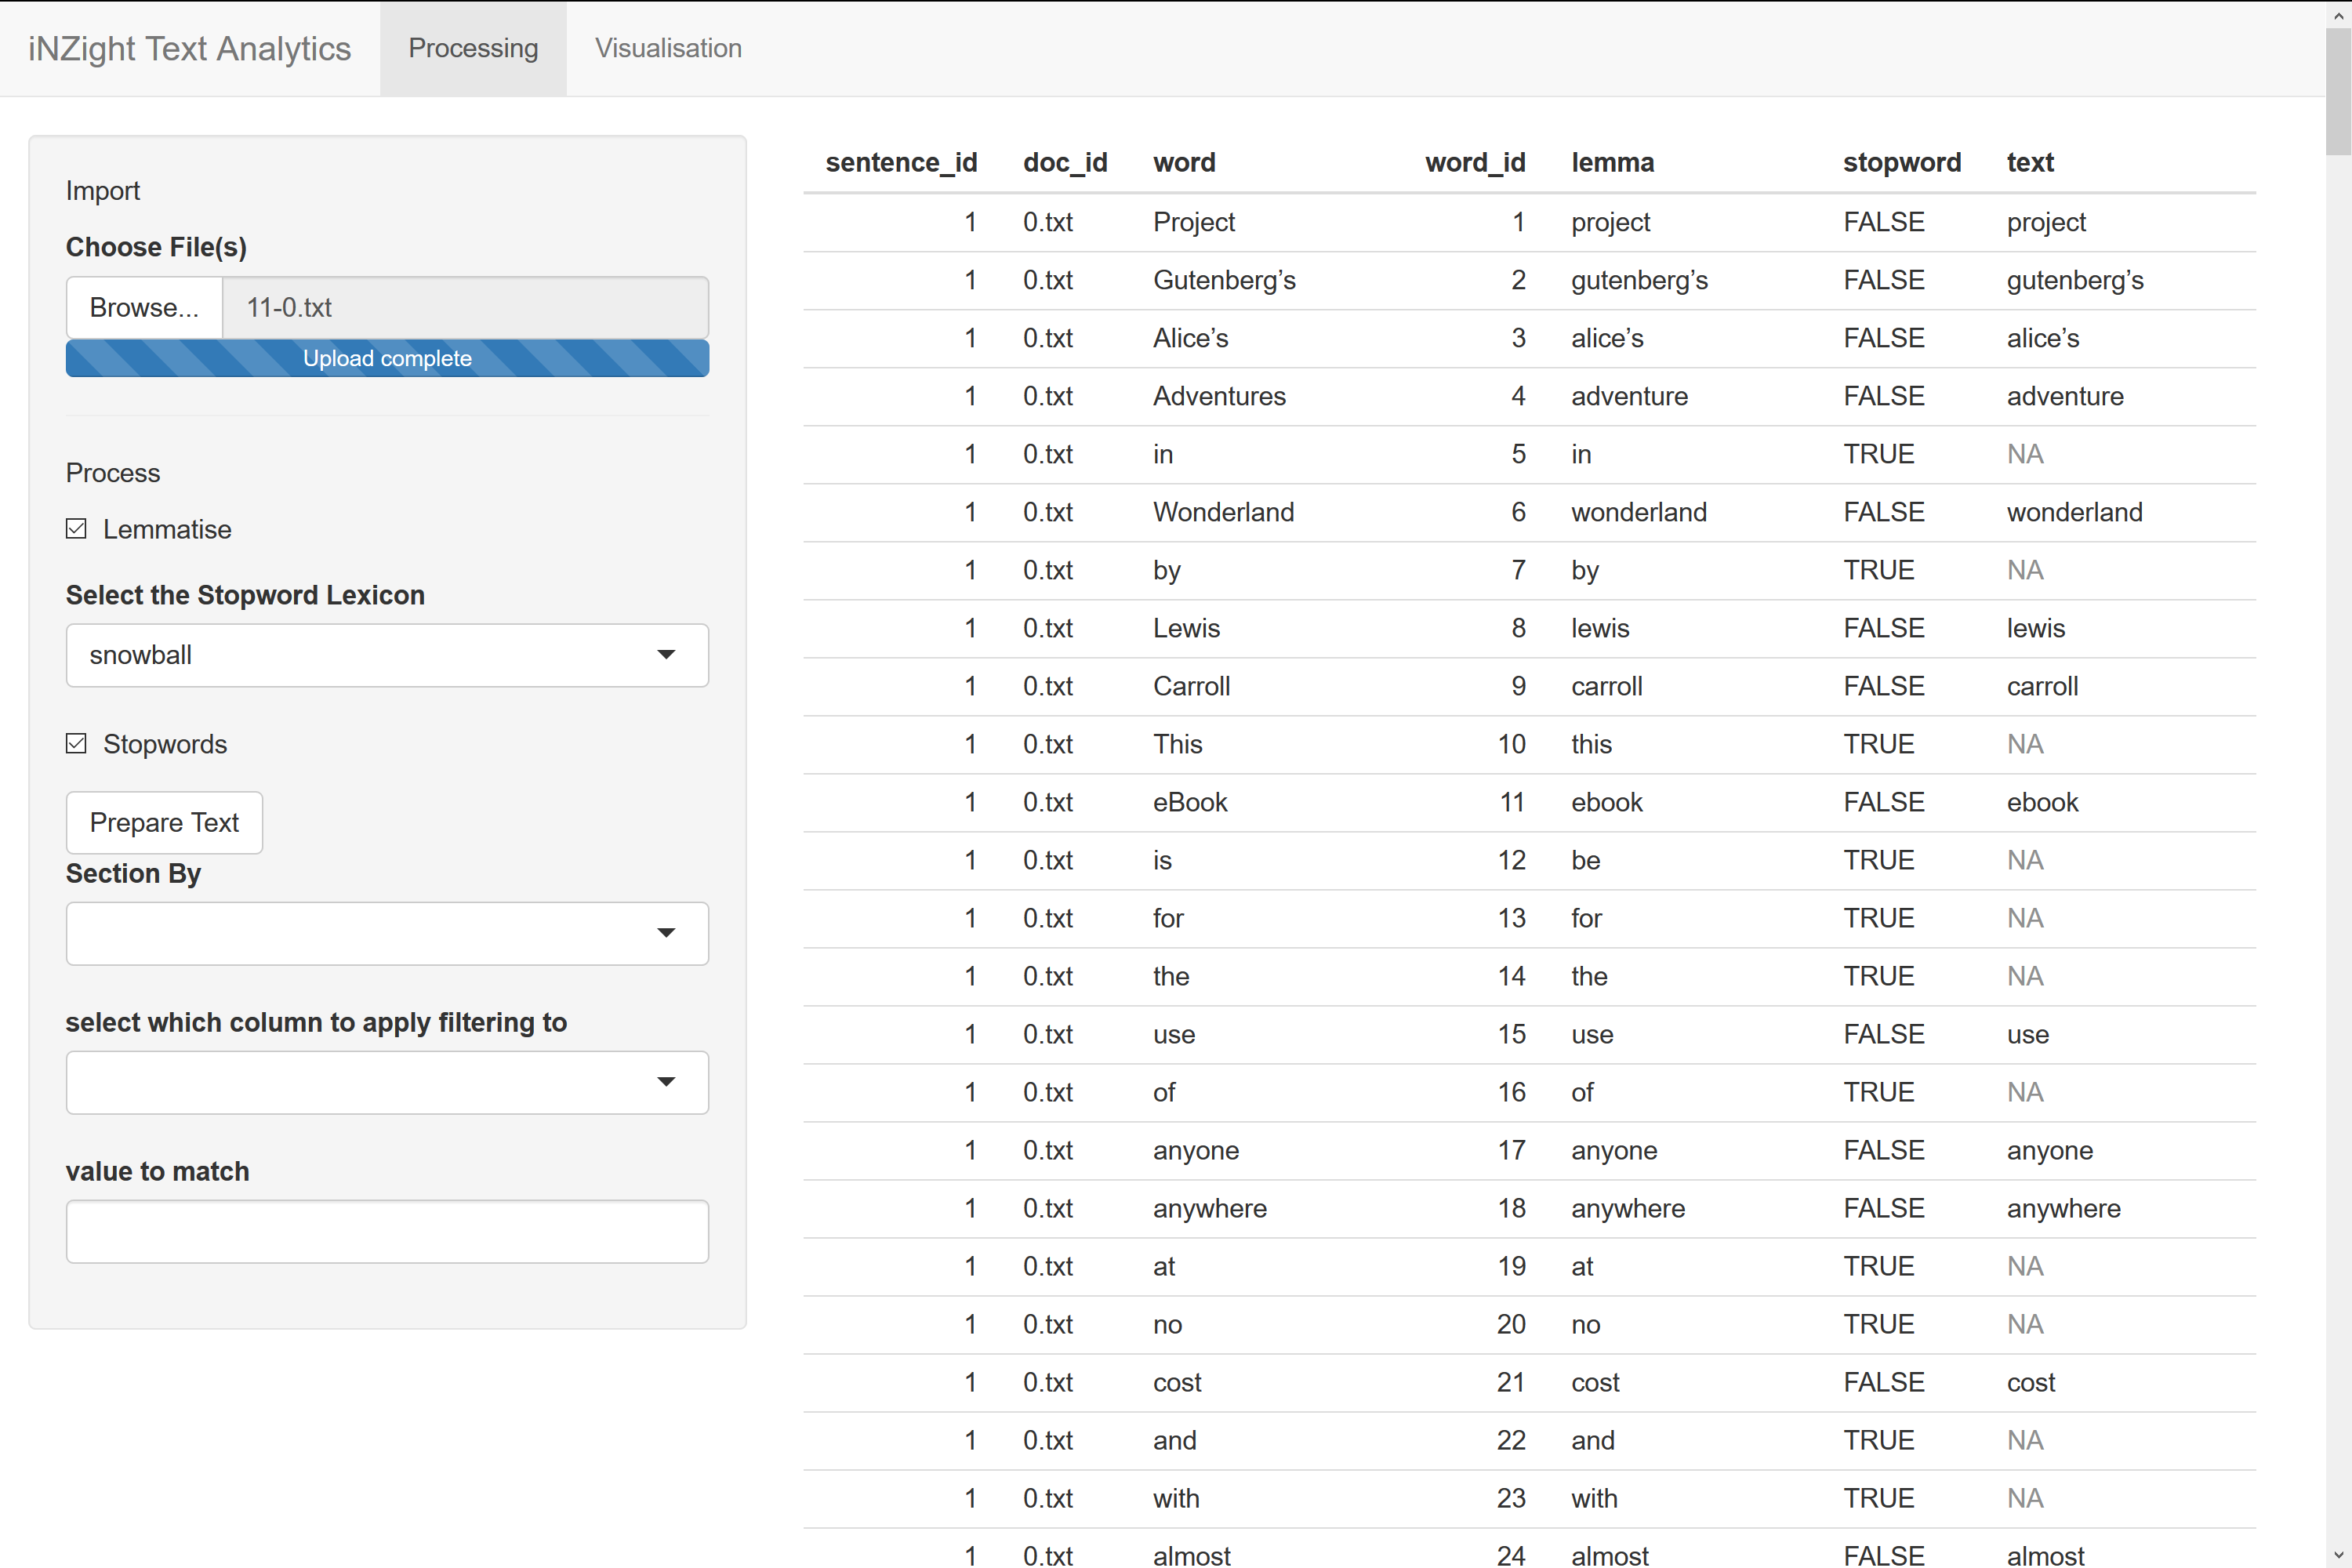
\includegraphics[scale=0.35]{processing-overview.png}
  \caption{Processing screen\label{fig:processing-overview}}
\end{figure}

\subsection{Importing}\label{sec:importing}

Text must first be brought in from an outside source to be useful for
the program. The import functions are such that all text from
different files exist in dataframes of equivalent structure. The
primary differences are that each row of an imported \texttt{txt} file
corresponds to a single line, whereas each row of an imported tabular
file corresponds to the row of the tabular file. Importantly for
tabular files, the column of the text intended for analysis must
currently be given the header of ``text'' prior to import. This
condition will be relaxed later. Of note is that importing of files is
a mostly solved problem in R, and most of the import functions in this
package are simple wrappers that serve the main role of standardising
the output. In the web app, importing occurs first, immediately prior
to processing, with a file browse button and a loading bar
(\underline{\cref{fig:processing-import-pro}})

\begin{figure}
  \centering
  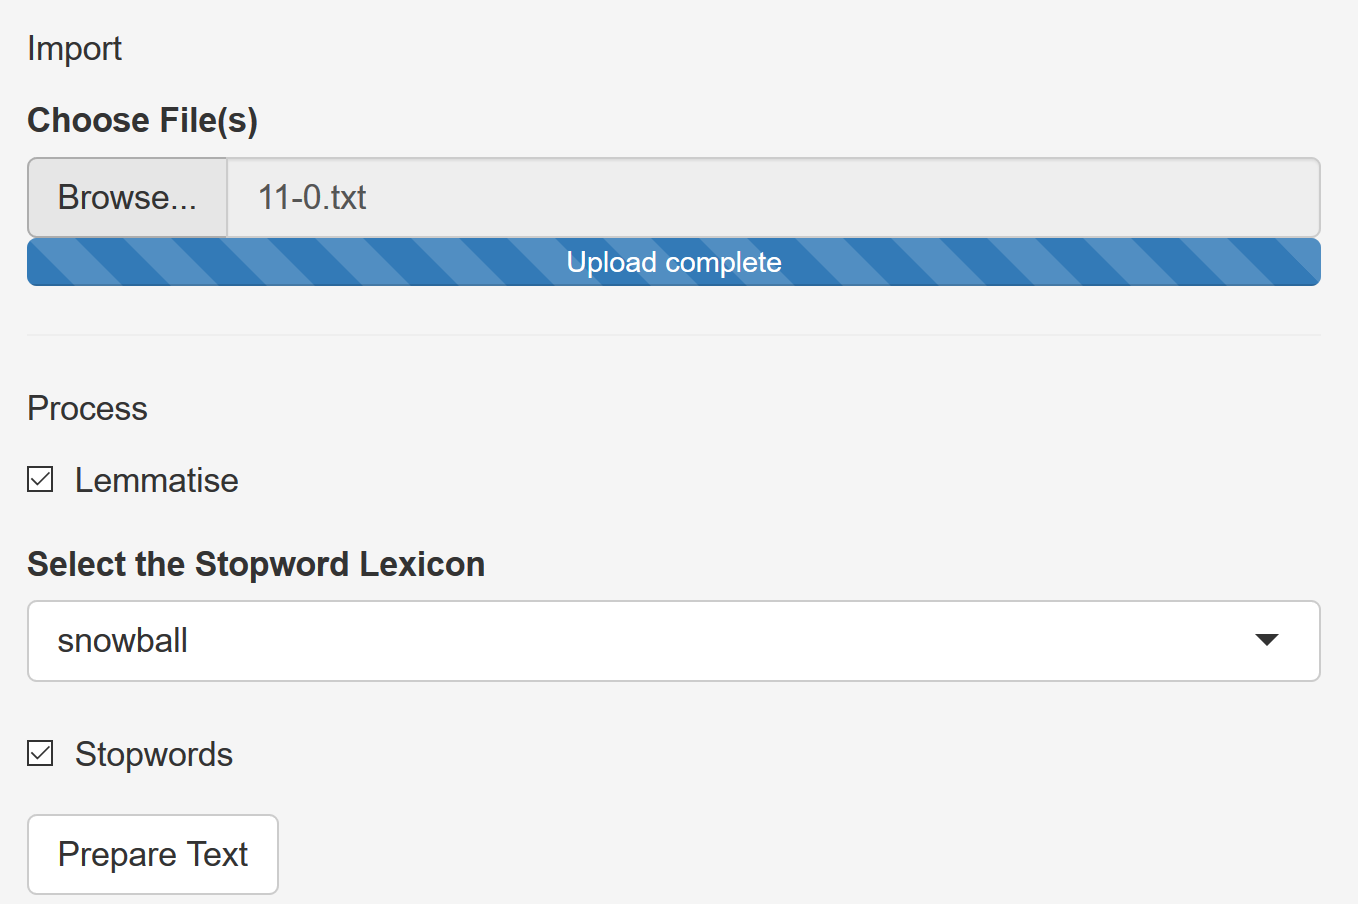
\includegraphics[scale=0.7]{processing-import-process.png}
  \caption{Importing a document\label{fig:processing-import-pro}}
\end{figure}

\subsubsection{Import \texttt{txt}}

The simple function \mintinline{r}{import_txt()}
(\underline{\cref{lst:import-txt}}) used to import \texttt{txt} files
simply reads lines from a file, and converts the data into a
tibble\autocite{muller19tib}, with a single column named ``text'' and
single row containing the document as a long string.

\subsubsection{Import \texttt{csv}}

CSV is a plaintext tabular format, with columns typically delimited by
commas, and rows by new lines. A particular point of difference in the
importation of tabular data and regular plaintext is that the text of
interest for the analysis should be (as per tidy principles) in one
column, with the rest being additional information that can be used
for grouping or filtering. Thus, additional user input is required,
namely the specification of which column is the text column of
interest. The function \mintinline{r}{import_csv()}
(\underline{\cref{lst:import-csv}}) is a simple wrapper around
\mintinline{r}{readr::read_csv()}\autocite{wickham18red}, created only
to maintain consistent naming conventions.

\subsubsection{Import Excel}

Much data exists in the Microsoft Excel format, and this must be
catered for. As tabular data, it is treated equivalently to
\texttt{csv}, with the function \mintinline{r}{import_excel()}
(\underline{\cref{lst:import-excel}}) being a wrapper
around \mintinline{r}{readr::read_excel()}.

\subsubsection{Import Wrapper for Arbitrary Number of Files}

To have just one function required to import files, two sub-functions
(\underline{\cref{lst:import-files}}) are defined;
\mintinline{r}{import_base_file()} imports any file, and
\mintinline{r}{import_files()} makes use of the aforementioned, to
import multiple files. The import of multiple files is no trivial
task; the program must shape them in such a way that they retain
identification, and fit into the same data structure together.
Different filetypes can be combined in the same analysis.

The base wrapper function takes in the filename, and other relevant
information, handling the importation process. It also stamps in the
name of the document as a column.

The base file import is generalised to multiple files with a multiple
import function: this will be our sole import function.

\subsection{Object Preparation}

From the imported files, their representations are transformed into a
lossless and efficient data structure that any analysis can make use
of, with a single function, \mintinline{r}{text_prep()}
(\underline{\cref{lst:text-prep}}). Our solution to the essential
constraint of losslessness is to separate and identify rows by each
word in a dataframe. The identification includes the line ID, the
sentence ID, and the word ID, producing a dataframe that takes the
form of \underline{\cref{tab:data-base}}.

\begin{table}[h]
  \centering
  
  \begin{tabular}{rrrl}
    line\_id & sentence\_id & word\_id & word\\
    \toprule
    1 & 1 & 1 & the\\
    1 & 1 & 2 & quick\\
    2 & 1 & 3 & brown\\
  \end{tabular}  
  \caption{Primary data structure format}\label{tab:data-base}
\end{table}

The reason for the ID columns is the preservation of the structure of
the text; If required, the original text, or chunks of it, can be
reconstructed in entirety, sans minor punctuation differences. The
options for the function in-app are given as checkboxes and dropdowns.

\subsection{Filtering}

Filtering of text is implemented directly with the
\mintinline{r}{dplyr::filter()} function, directly in the server of
the Shiny app. Filtering can take place multiple times throughout an
analysis. The program is flexible enough such that after some initial
analytics have been done in the insight layer, preparation can be
returned to and the text can be filtered based on features seen in the
analytics.

\subsection{Lemmatisation}

Lemmatisation is the process of transforming words into their
dictionary form. It is a very complex, stochastic procedure, as
natural languages don't follow consistent and clear rules all the
time. Hence, models have to be used. Despite the burden, it is
generally worthwhile to lemmatise words for analytics, as there are
many cases of words not being considered significant, purely due to
taking so many different forms relative to others. Additionally,
stopwords work better when considering just the lemmatised form,
rather than attempting to exhaustively cover every possible form of a
word.

\texttt{textstem} is an \texttt{R} package allowing for easy
lemmatisation, with it's function
\mintinline{r}{textstem::lemmatize_words()} transforming a vector of
words into their lemmatised forms (thus being compatible with
\mintinline{r}{dplyr::mutate()} straight out of the
box)\autocite{rinker18}. The lemmatisation in this program is managed
entirely by this single function in the server end of the Shiny app.
The package udpipe was another option, but it requires downloading
model files, and performs far more in-depth linguistic determinations
such as parts-of-speech tagging, that at this point are excessive. It
is worth noting that, as with stopwords, there are different
dictionaries available for the lemmatisation process, but we only use
the default, as testing has shown it to be the simplest to set up and
just as reliable as the rest.

\subsection{Stemming}

Stemming is the removal of word endings, and is far simpler than
lemmatisation. For example, lemmatisation may change the word
``happiness'' to ``happy'', while stemming would change it to
``happi'', removing the ``ness''. This doesn't require as complex a
model, as it is fairly deterministic. Stemming is not always as
effective as lemmatisation, as the base word ending is not
concatenated back on at the tail, so all that remains are ``word
stumps''. However, it may sometimes be useful when the lemmatisation
model isn't working effectively, and \texttt{textstem} provides the
capability with \mintinline{r}{textstem::stem_words()}. We have not
implemented this yet, as it is not as essential to an analysis when
lemmatisation is already available.

\subsection{Stopwords}\label{sec:stopwords}

The package makes use of dictionary-form stopwords, allowing for the
input of both developed lexicons as well as user input. Two functions
(\underline{\cref{lst:stopwords}}) compose stopwords:
\mintinline{r}{get_sw()}, which gathers user input, queries the
selected lexicon and combines the two, and
\mintinline{r}{determine_stopwords()} which adds a boolean
\mintinline{r}{TRUE | FALSE} column to the input dataframe. The
stopwords functions operate on the original text, but if lemmatisation
has been performed, then the functions operate on the lemmatised
forms.

\subsection{Formatting}\label{sec:formatting}

The final component in preparation is to format the prepared object
with the correct attributes which allow formatting to be automated. A
wrapper named \mintinline{r}{format_data()}
(\underline{\cref{lst:format-data}}) is defined that takes all
combinations of stopwords and lemmatisation options and intelligently
connects them to create the ``insight column'' in a dataframe, when
insight functions are applied later on in the pipeline. For the
purpose of standard interoperability, e.g., with the \texttt{ggpage} package,
this column is named ``text''.

At the heart of this function is an \mintinline{r}{ifexp()} that
encodes the following logic involving the interaction of stopwords and
lemmatisation, to enable the correct output text based on stopword and
lemmatisation options, as given in \underline{\cref{tab:formatting}}.

\begin{table}[h]
  \centering
  \begin{tabular}{p{20mm}|p{50mm}p{50mm}}
    & Stopwords True                                                                                    & Stopwords False                      \\
    \toprule
    Lemmatise True  & Lemmatise, determine stopwords on lemmatisation, perform insight on lemmas sans stopwords         & Lemmatise, perform insight on lemmas \\
    Lemmatise False & Determine stopwords on original words (no lemmatisation), perform insight on words sans stopwords & Perform insight on original words    \\
  \end{tabular}
  \caption{Formatting Logic for Stopwords and
    Lemmatisation}\label{tab:formatting}
\end{table}

Based on the combination, stopword filtering and lemmatisation take
place inside the function.

\subsection{Sectioning}

Plain text, as might exist as a Gutenberg download, differs from more
complex representations in many ways, including a lack of sectioning
--- for example, chapters require a specific search in order to jump
to them. A closure, \mintinline{r}{get_search()}
(\underline{\cref{lst:section}}) is composed that searches text based
on a regular expression intended to capture a particular section.
Several search functions have been created from that closure, such as
\mintinline{r}{get_cantos()}, \mintinline{r}{get_sections()}, etc. The
sections are added to the dataframe with \mintinline{r}{section()}.
These have been given as a drop-down selection list in the app (date,
advanced users could be given the option to compose their own regular
expressions for sectioning.

\begin{figure}
  \centering 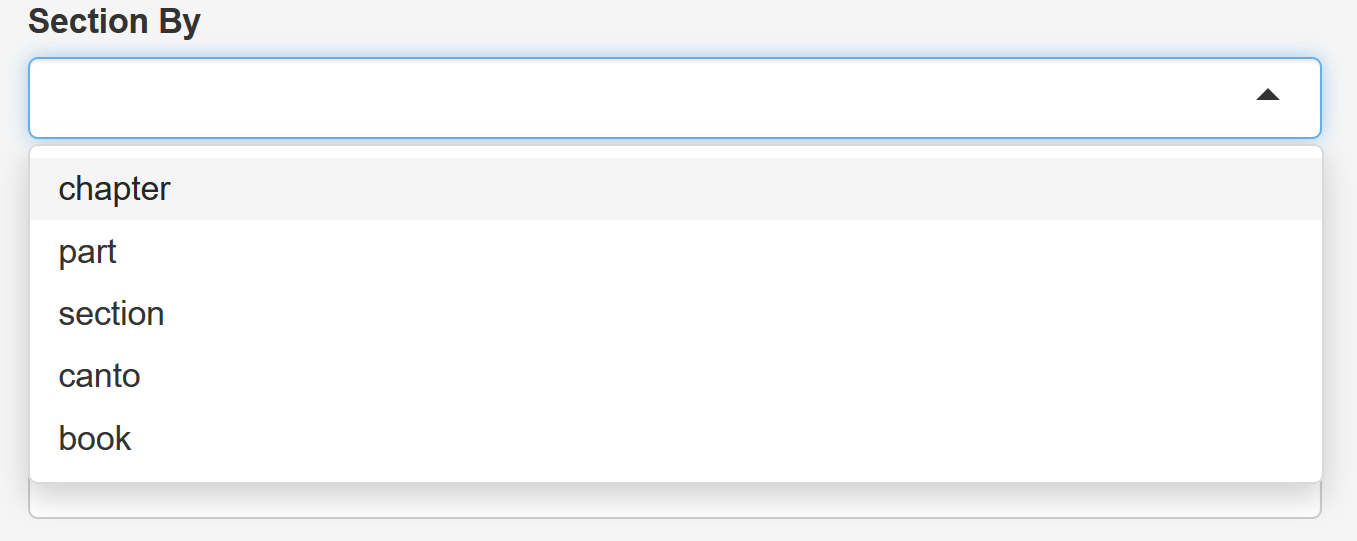
\includegraphics[scale=0.7]{processing-section.png}
  \caption{Section types\label{fig:processing-section}}
\end{figure}

\subsection{Grouping}

Grouping is an essential, killer feature of the app. The
implementation makes use of a \mintinline{r}{dplyr::group_by()}
command in the Shiny server on the prepared object, over
user-specified groups, and all further insights and visualisations are
performed groupwise. This allows for immediate and clear comparisons
between groups.

Like filtering, after some initial analytics have been done in the
insight layer, preparation can be returned to, and a new variable
constructed based upon the initial analytic results, so the the text
can be grouped-on based on the the features seen in the analysis.

\section{Insight}\label{sec:insight}

After processing has yielded an appropriate data structure to operate
upon, analytic functions may be performed, under the banner of
``insight''. The bulk of this package is composed of the insight
functions, divided into term insights, and higher level (aggregate)
insights. Higher level insights exist where units of analysis may be
n-grams, sentences, chapters, documents, etc. Additional functionality
is very easy to implement, just requiring a named function that can
operate on the standard data structure. The output of an insight
measure is added as an additional column to the dataframe resulting
from processing the text.

\subsection{Term Insight}\label{sec:term-insight}

Individual words form the basis of any analysis, and reveal a great
amount of information about a text. Term insights all have the same
expected form of input an output, with the output vector always
matching the size of the input vector, with elements being a direct
element-wise mapping.

\subsubsection{Term Frequency}\label{sec:term-frequency}

Frequencies of words are useful in getting an understanding of what
terms are common in a text. This is one insight in particular that
usually requires stopwords to have been previously removed, otherwise
the top words will always be syntactical glue, such as articles. A
function named \mintinline{r}{term_freq()}
(\underline{\cref{lst:term-freq}}) is defined to perform this
analysis. Running this function with stopwords left in is a good
comparative diagnostic for checking whether the stopword lexicon is
removing words that aren't intended to be removed.

\subsubsection{n-Grams}\label{sec:n-grams}

One difficulty that presents itself in the determination of n-grams is
the treatment of missing words. Stopwords have to be considered, lest
the original text be altered destructively. An example of this
difficulty is through the two sentences, ``I went to the shops'', and,
``I went to the car''. Most stopword lexicons would remove all words
but ``went'', ``shops'', and ``car''. This leaves a grey area ---
should the n-grams make reference to the missing values, or skip over
them?

This was answered in this package by the slightly more difficult to
implement skipping-over of missing values, in the n-gram insight
function \mintinline{r}{get_ngram()}
(\underline{\cref{lst:get-ngram}}). This way, the results of the
analysis would not be polluted with ``NA'', as is the very intention
of stopword removal. An example of the expected output of this
procedure is given in \underline{\cref{tab:bigram-miss-val}}; each
element of the bigram column corresponds to the element in the list
column of the same row. n-grams are stored in this way to maintain the
data-frame structure.

\begin{table}
  \centering
  \begin{tabular}{lll}
    list & list shifted back & bigram \\
    \midrule
         & 1                 &        \\
    1    & 2                 & 1 2    \\
    2    & X                 & 2 4    \\
    X    & 4                 & X      \\
    4    & 5                 & 4 5    \\
    5    & X                 & 5 7    \\
    X    & 7                 & X      \\
    7    & X                 & X      \\
    X    &                   & X      \\
  \end{tabular}
  \caption{Bigram behaviour with missing values indicated by
    ``X''\label{tab:bigram-miss-val}}
\end{table}

The function is one of the only internally non-pure functions (through
changing state through for- and while- loops) in the entire package,
as searching sequentially along a list is far easier to conceive of in
imperative terms.

The frequency of a particular n-gram is given by applying the
\mintinline{r}{term_frequency()} function to the newly determined
n-gram column, in the \mintinline{r}{ngram_freq()} wrapper
(\underline{\cref{lst:get-ngram-freq}}). A typical
visualisation of n-grams is demonstrated in
\cref{fig:visualisation-n-gram-facet}.

\begin{figure}
  \centering
  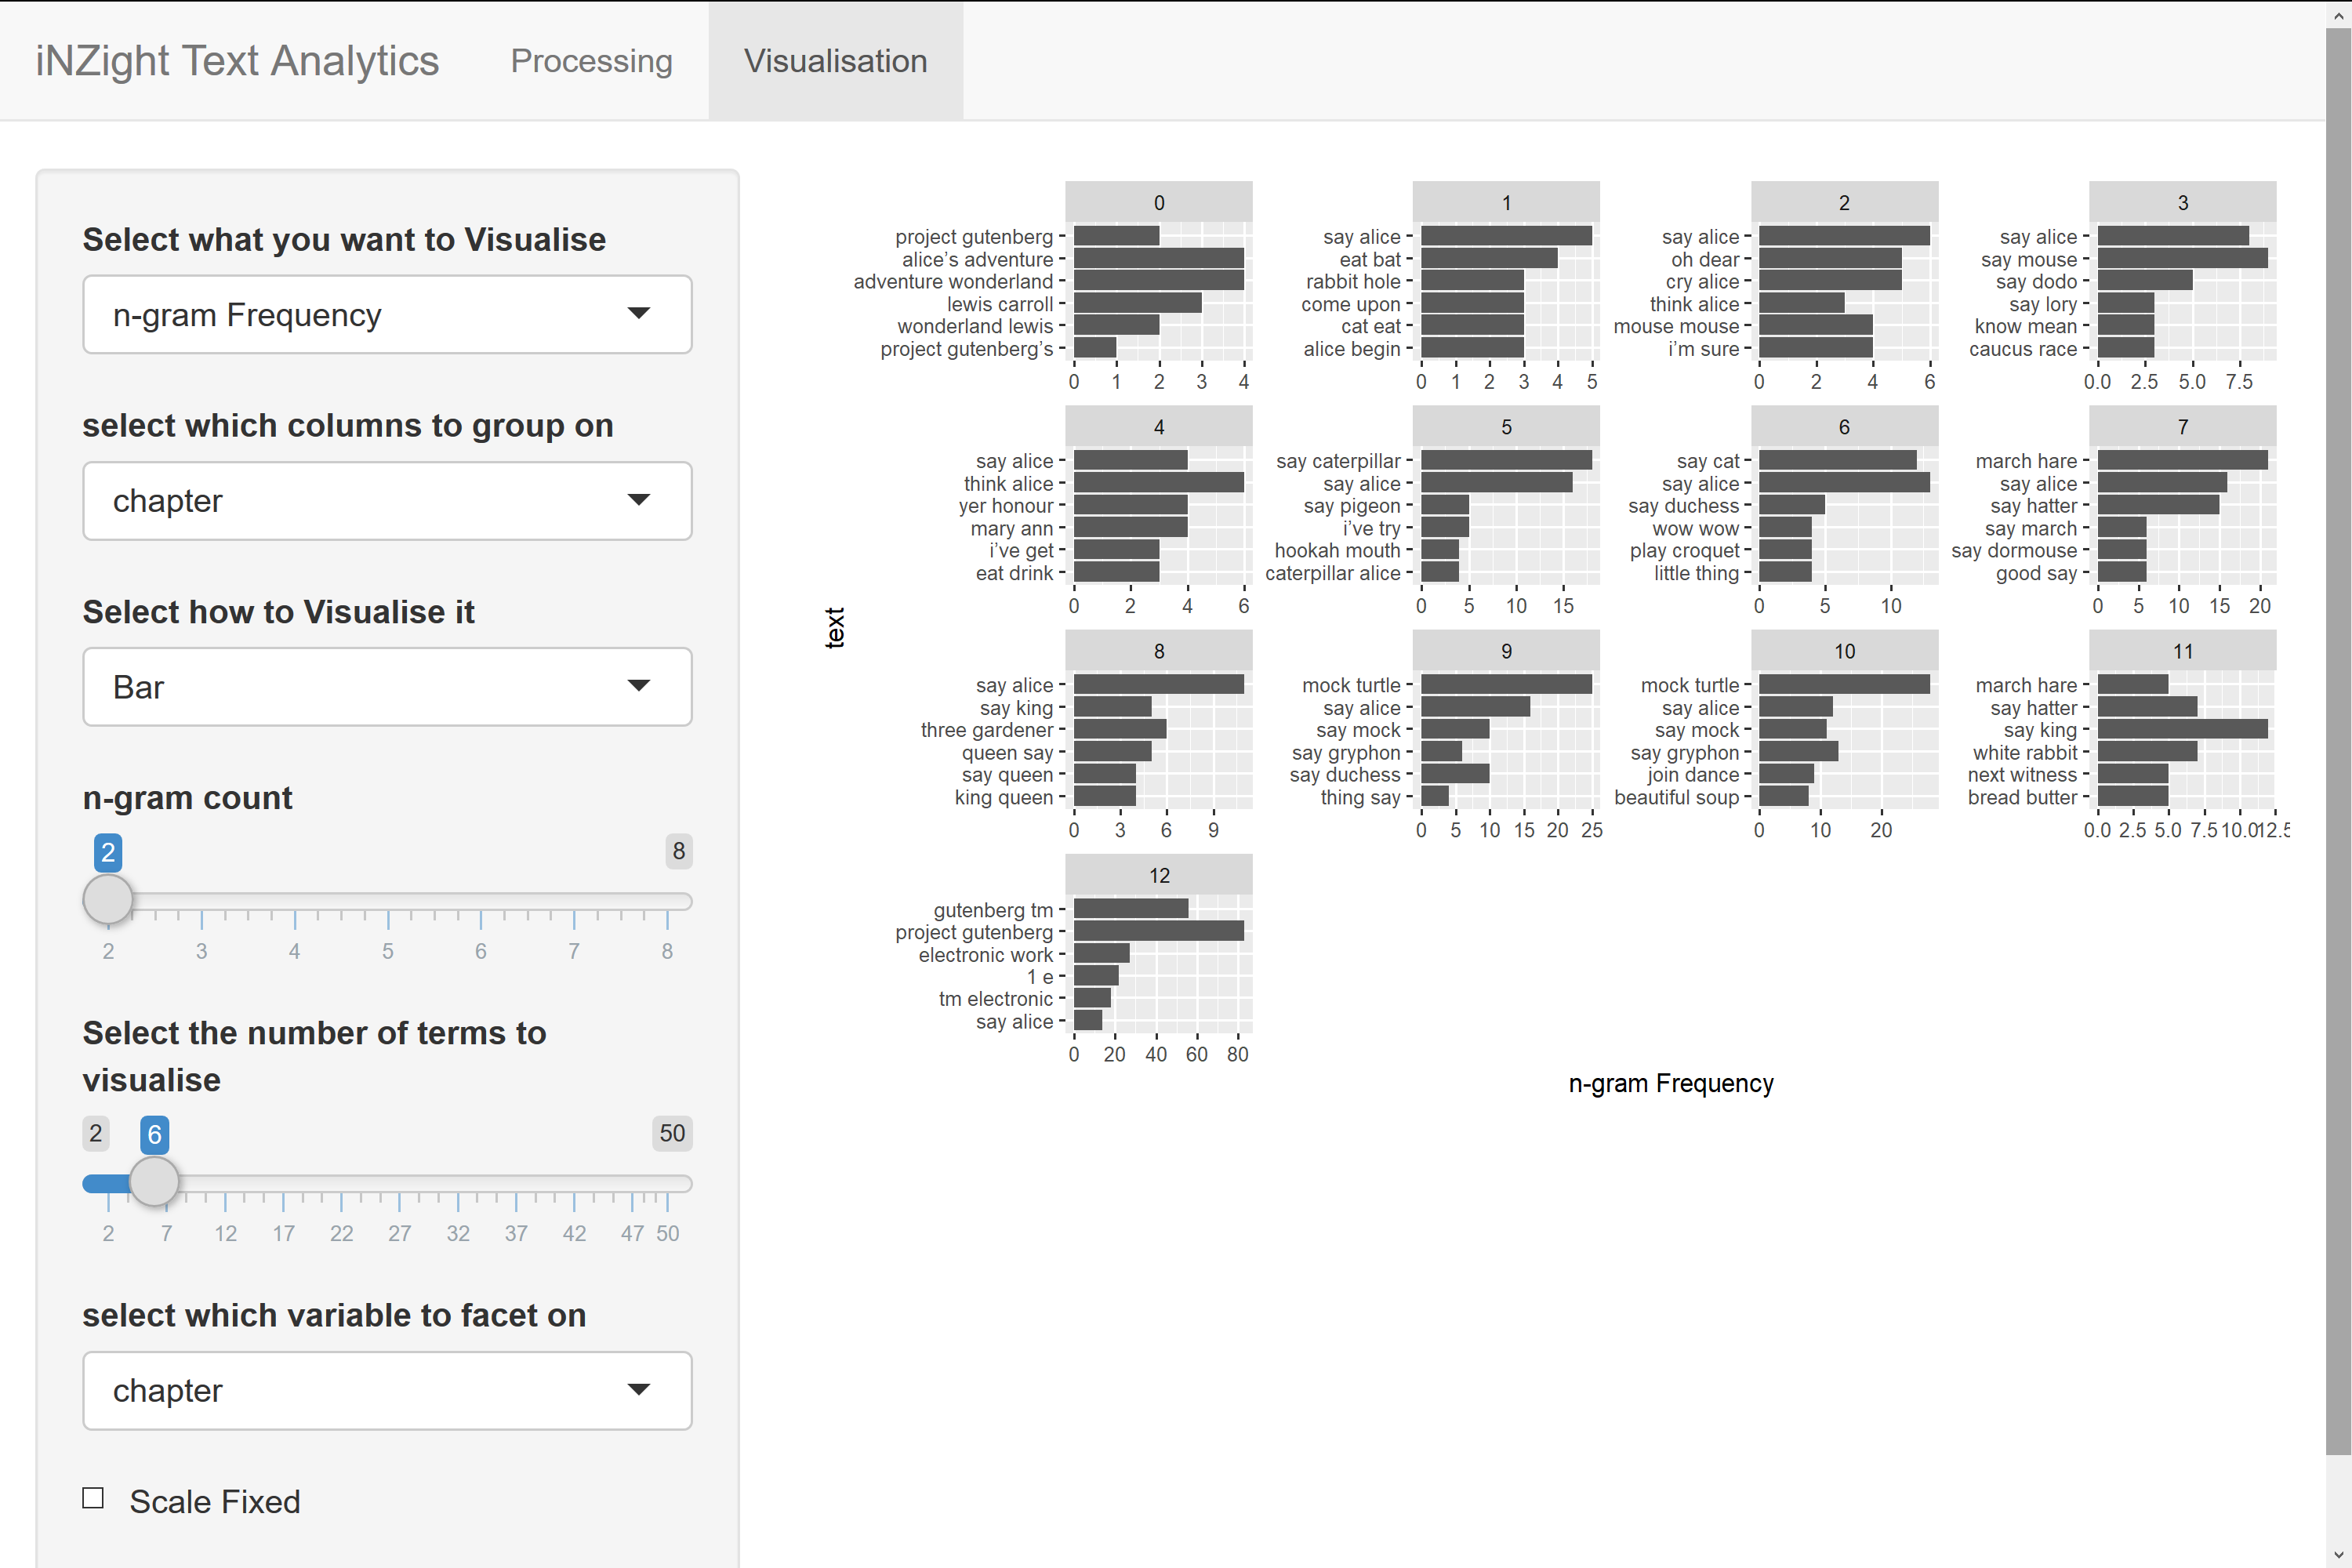
\includegraphics[scale=0.35]{visualisation-n-gram-facet.png}
  \caption{n-gram visualisation with facetting by
    chapter\label{fig:visualisation-n-gram-facet}}
\end{figure}

\subsubsection{Key Words}\label{sec:key-words}

Determination of key words is a useful analytic function that differs
from finding the most frequent words. Key word algorithms are
generally based on some derivative of the TextRank algorithm. This
algorithm constructs an adjacency matrix of a directed graph with
words or sentences as the nodes, and the arc weights reflecting some
measure of similarity between words, typically a function of
co-occurrence within the same sentence. The PageRank algorithm is run
on this graph, picking up the most representative words that may not
necessarily be the most frequent. The words with the highest PageRank
scores are then selected to produce a set of key words. A function
named \mintinline{r}{keywords_tr()} (\underline{\cref{lst:keywords}})
implements this, on the shoulders of the \mintinline{r}{textRank}
package\autocite{wijffels19}.

Of note is that all words other than stopwords are treated as
relevent, but the standard algorithm works better on data that has had
parts of speech tagging, typically assessing only nouns and
adjectives. This function doesn't make use of such tagging, as the
processing burden for Parts of Speech tagging is enormous and slow,
undercutting the necessity for the interactive app to be quick and
responsive. A faster, simplified version may be implemented in the
future.

\subsubsection{Term Sentiment}\label{sec:term-sentiment}

Term sentiment is one of the most common analyses, especially in the
automated processing of free-form survey responses. It gives some
measure of the sentiment of the terms in a text, giving insight into
the emotional charge of a text and it's structure.

Sentiment analysis can either make use of dictionaries, where each
word has an associated score, or models, where complexities such as
negation or amplification are considered. The function defined in this
package to determine term sentiment is named
\mintinline{r}{term_sentiment()}
(\underline{\cref{lst:term-sentiment}}). It currently makes use of the
simpler and less processing-intensive dictionary form. There are
numerous dictionaries available, giving numeric scores or
categorisations of sentiment type. As numeric scores are the easiest
to visualise, these have been the intended implementation of the
function. Well-regarded dictionaries (``lexicons'') include ``AFINN'',
which gives a numeric score centred at zero, ``bing'', which gives a
classification of the emotional category, and ``ISO''. The default of
this program is the lexicon ``AFINN''.

A problem in dictionary methods for sentiment analysis is that the
same word may or may not carry a perticular emotional charge,
depending on the subject area and type of writing. Specialised
dictionaries exist for some specialist subject areas, which aim to
remedy this. For example, in mathematics, a ``problem'' has very
different emotional connotations to a ``problem'' in the diagnosis of
a hospitalised patient.

The function currently possesses a strong dependency on the \texttt{tidytext}
package. This has come at a cost, with \texttt{tidytext} having a constantly
changing and unreliable API --- future development will move away from
such a dependency. At present (though not at the time of original
inclusion), the \texttt{tidytext} package requires download of sentiment
dictionaries through the command line at first use, which is an
annoying impediment in a GUI application.

\subsubsection{Moving Average Term
  Sentiment}\label{sec:moving-average-term}

A statistical summary of a sentiment in time gives a more contextual
picture of how sentiment is given in a text. The function defined as
\mintinline{r}{ma_term_sentiment()}
(\underline{\cref{lst:ma-term-sentiment}}) performs such a task and is
flexible enough to take any statistic or lag, defaulting to be a
moving average of 10. The first \mintinline{r}{lag} terms will be
\mintinline{r}{NA}, and the number of \mintinline{r}{lag} is
inclusive, matching the semantics of R's indexing starting at 1.
Moving Average Term Sentiment finds a natural visualisation as a time
series plot, demonstrated in
\underline{\cref{fig:visualisation-ma-overview}}.

\begin{figure}
  \centering
  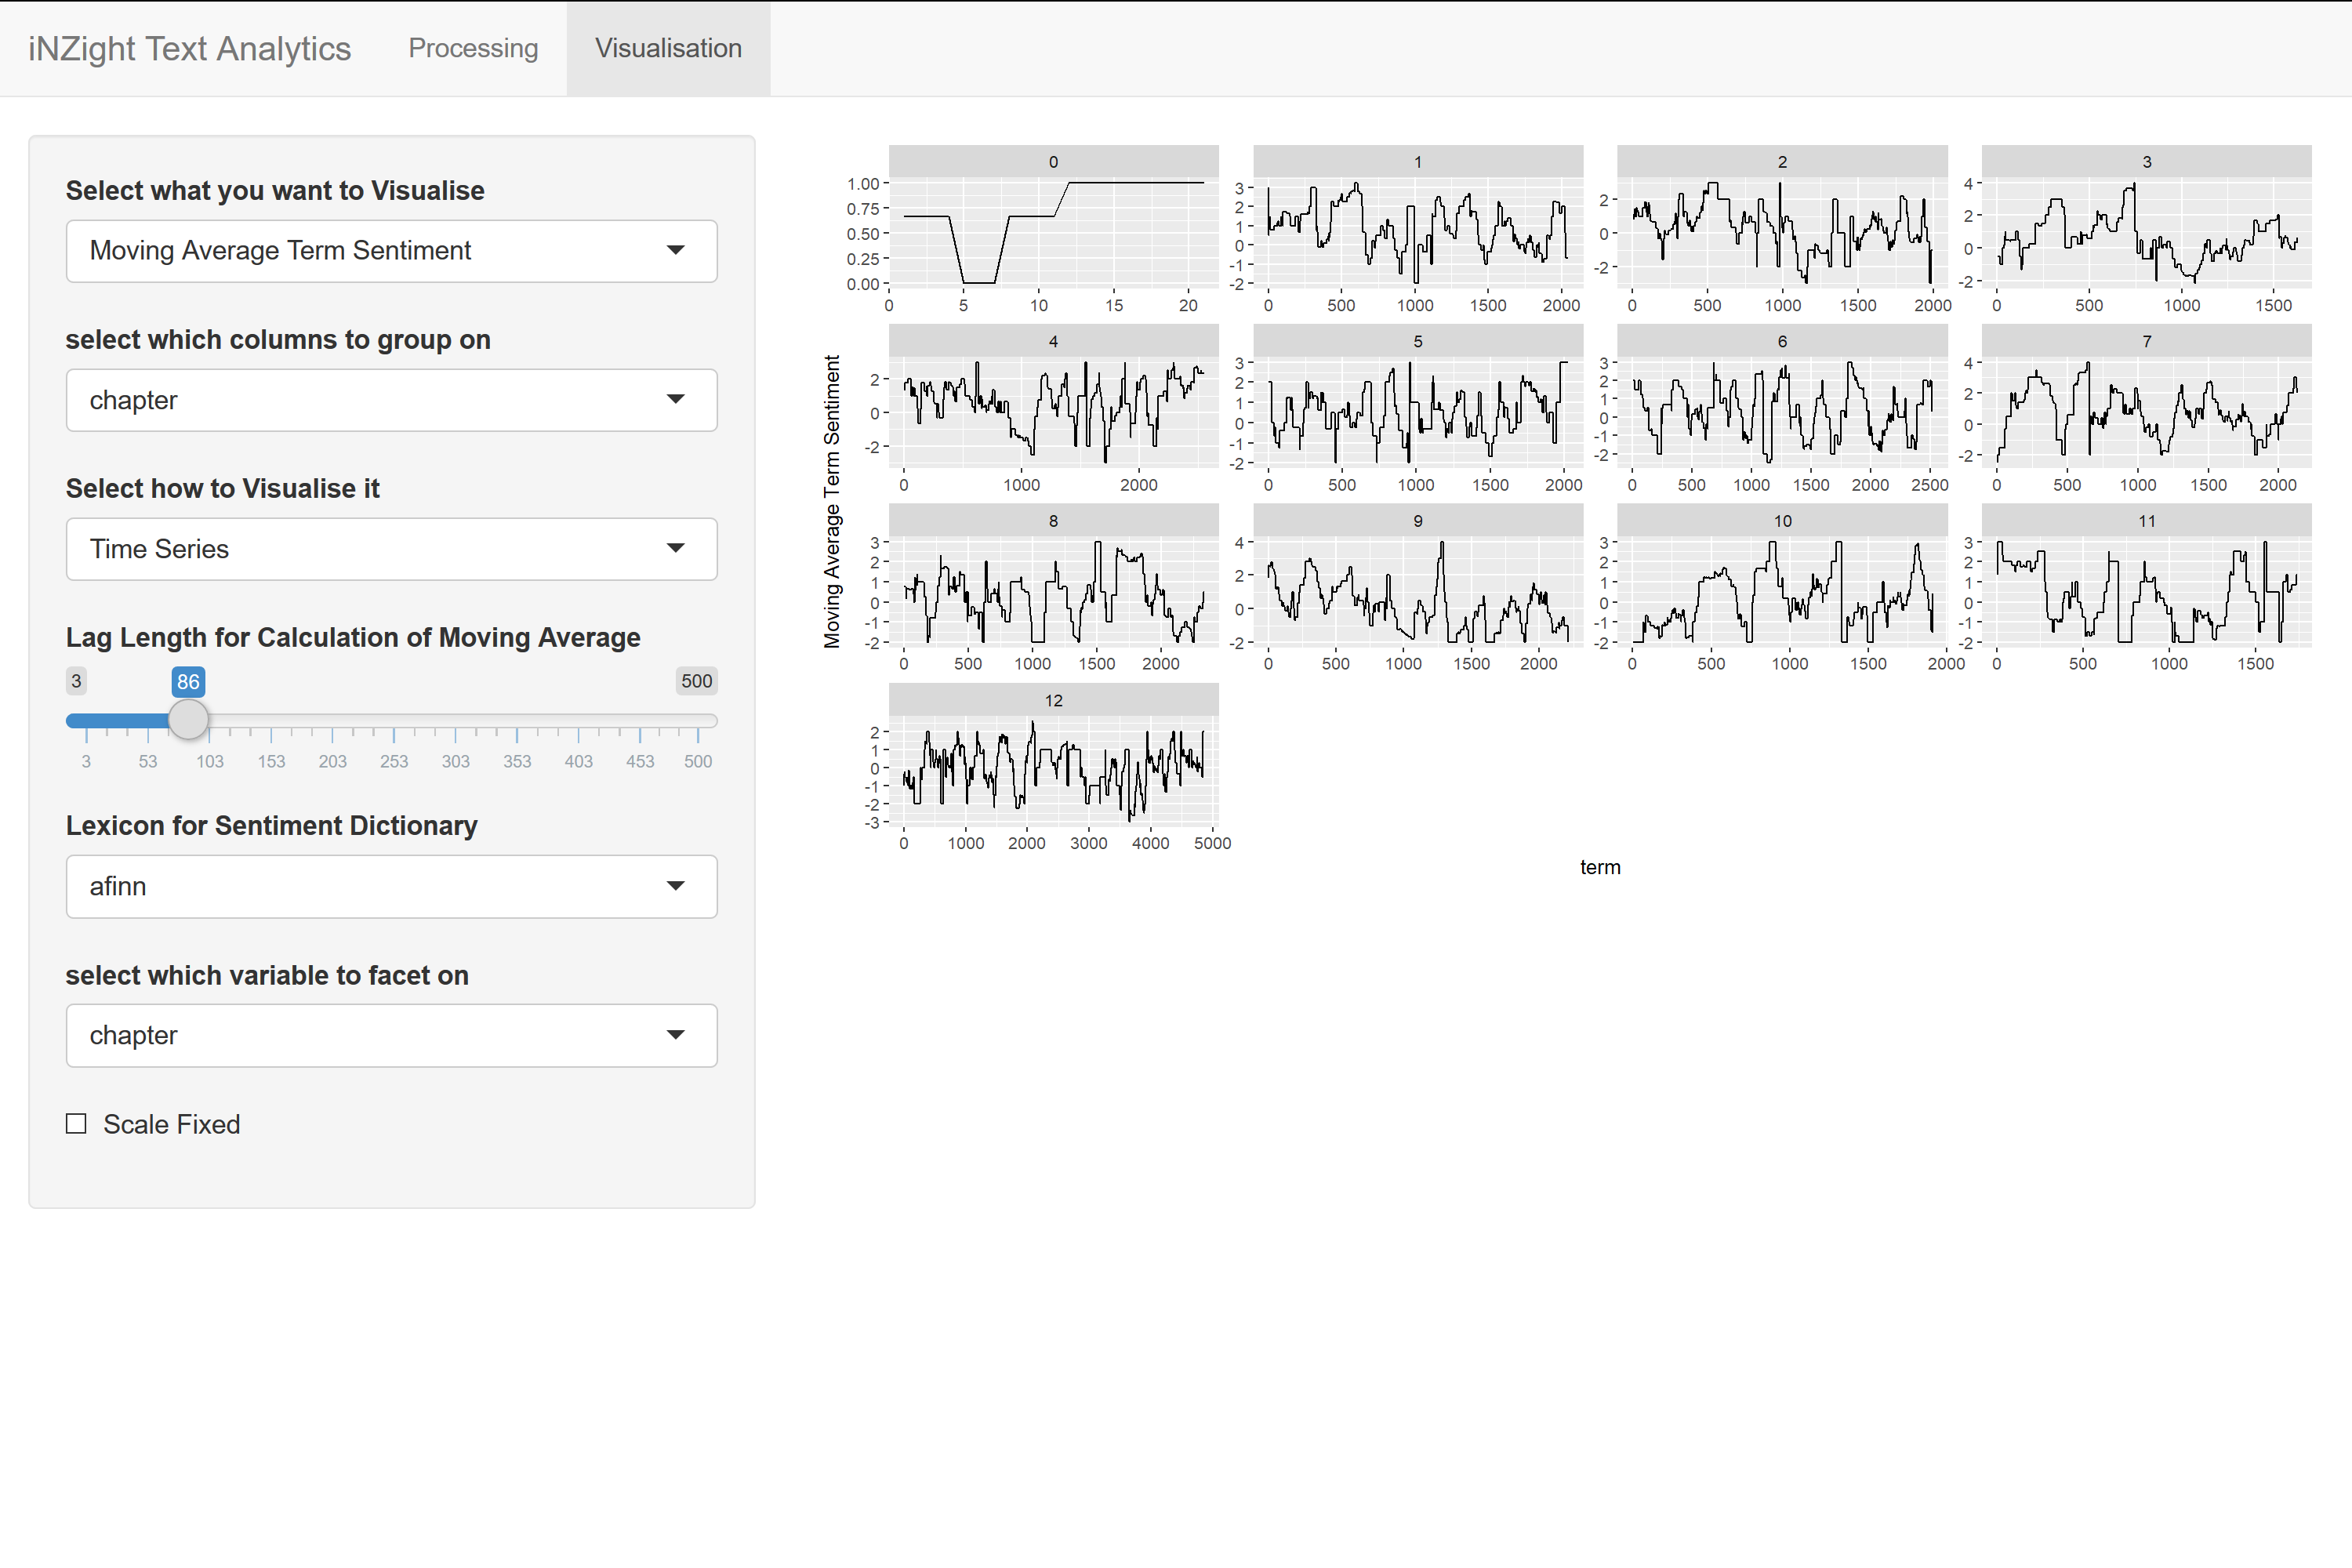
\includegraphics[scale=0.35]{visualisation-ma-overview.png}
  \caption{Moving average term sentiment visualised with Time
    Series\label{fig:visualisation-ma-overview}}
\end{figure}

\subsection{Aggregate Insight}\label{sec:aggregate-insight}

Analysis is not just restricted to words alone, and can consider the
emergent forms composed through collections of words, such as
sentences and documents, even tweets or responses. With a \texttt{csv}
input file, aggregates can be also be defined in columns corresponding
to the text column, and made use of through the following functions.
All functions perform similarly to the term-level insight functions,
with vectors as input and vectors as output. The aggregate functions
also require another vector defining aggregate groupings, in a similar
manner to the \mintinline{r}{INDEX} argument of
\mintinline{r}{tapply()}.

\subsubsection{Term Count}\label{sec:term-count}

Word count on some aggregate group follows the pattern where the
simpler a function is, the more analytical power it seems to give. A
function named \mintinline{r}{term_count()}
(\underline{\cref{lst:term-count}}) is defined to count terms per
grouping. The typical usage for this would have an aggregation over
sentence ID, giving the word count in each sentence. This can be used
in conjunction with grouping, allowing for a hierarchical measure of
the distribution of, for example, sentence lengths per chapter within
a document. If these markedly differ between one chapter and the rest,
there is likely a different author or style in that one chapter.

Note in the function the near canonical example of
split-apply-combine, or MapReduce style. This will allow for major
performance gains if parallelised, ideal for the large datasets
typically made use of in text analytics.

\subsubsection{Key Sections}\label{sec:key-section}

Often keywords aren't very explanatory on their own; patterns only
really develop in the aggregate. Determining key sections aggregating
over sentence reveals the most representative sentences in a document.
As such, it is a form of automated summarisation. A function named
\mintinline{r}{key_aggregates()} is given to compute such an analysis
(\underline{\cref{lst:key-sections}}). LexRank is used as the default
algorithm for finding key-sentences, as testing has demonstrated that
textrank takes too long, though LexRank still takes a long time for
processing\autocite{spannbauer19}. In testing this function, it was
run over the original paper describing LexRank, with the results being
a very efficient summary of the paper, outlining the key notions
behind the algorithm.

LexRank is essentially the same as TextRank, however it uses cosine
similarity of Tf-Idf vectors as it's measure of similarity. LexRank is
better at working across multiple texts, due to the inclusion of a
heuristic known as ``Cross-Sentence Information Subsumption (CSIS)''.

Testing shows a performance of around 3--4 minutes for
\(\approx 30,000\) words of text aggregated over \(\approx 3000\)
sentences. This is not terrible performance for a graph-traversing
algorithm, but a warning is definitely required at the user end.

\subsubsection{Aggregate Sentiment}\label{sec:aggregate-sentiment}

Like the added context that key sentences bring over key words, a
similar situation is true of sentiment. A function named
\mintinline{r}{aggregate_sentiment()}
(\underline{\cref{lst:aggregate-sentiment}}) is given to determine a
statistic of sentiment over some group; most commonly, the mean
sentiment of each sentence or ``response'' in a text. This function is
higher-order, and can deliver any statistic of a group's sentiment;
mean, median, variance etc. Importantly, this function will only work
with numeric sentiment lexicons, with AFINN as the default.

\subsubsection{Word Correlation}\label{sec:word-correlation}

Word correlation provides a measure of relation between two words,
typically based on their existence in sentences together. This is the
word-level insight that is the most difficult-to-implement in an
efficient manner, due to the requirements that the dataframe remains
tidy and lossless. It would be impractical to have as the columns
every word with every correlation score to every other word. The
solution conceived of for this is by taking input from the user to
specify words, giving a vector of correlations between every other
word in the text and the specified word, with element-wise
correspondence between words in the text and the correlation
coefficients. The best form of visualisation would be individual words
with their scores, a correlation matrix for some words, or a table and
search. \mintinline{r}{widyr} implements a
\mintinline{r}{widyr::pairwise_cor()} function, however it appears to
determine the correlations of every single word with each other,
creating a far larger object than what is
needed\autocite{robinson19:widyr}. Implementation will likely have to
be performed from scratch in the future, unless an appropriate package
is found.

\subsection{Wrapper}\label{sec:wrapper}

The insights of choice can all be combined into a wrapper function
\mintinline{r}{get_insight()} (\underline{\cref{lst:get-insight}}),
taking the forms and arguments of the insights and applying those
chosen. Two separate functions were created for the careful handling
of term and aggregate insight. Initially these functions made use of
an \mintinline{r}{eval(parse())} style of evaluation, however this
proved to be too unclear in communicating the function capabilities,
and was changed to a table of functions that could be called. The loss
in power was justified by the gain in clarity.

The losslessness of the data structure created finds it's strengths in
the function \mintinline{r}{bind_aggregate()}
(\underline{\cref{lst:bind-aggregate}}), which recreates the original
text structure based on some aggregation, such as sentence ID.\

\section{Visualisation}\label{sec:visualisation}

Visualisation is extremely useful in the communication of text
analysis, and often forms the end-point of much of the automated
analysis. Development has grouped visualisations by their output
intention, rather than by their implementation, as part of the
single-responsibility principle, to be ends-focused rather than
means-focused. All of the visualisations in this package make heavy
use of \mintinline{r}{ggplot2}, due to the ease of facetting plots
based on grouping variables. The ``Grammar of Graphics'', which ggplot
is based upon, has not necessarily proved any more useful than the
base \texttt{R} plots for development purposes, with ease of facetting
and the excellent compatibility with Shiny being the principal reasons
for use.

Visualisation in the app consists of a full tab including options and
output (\underline{\cref{fig:visualisation-overview}}). Options vary
by type of insight selected, for example n-grams having unique options
related, as in \underline{\cref{fig:visualisation-n-gram-options}}.

\begin{figure}
  \centering 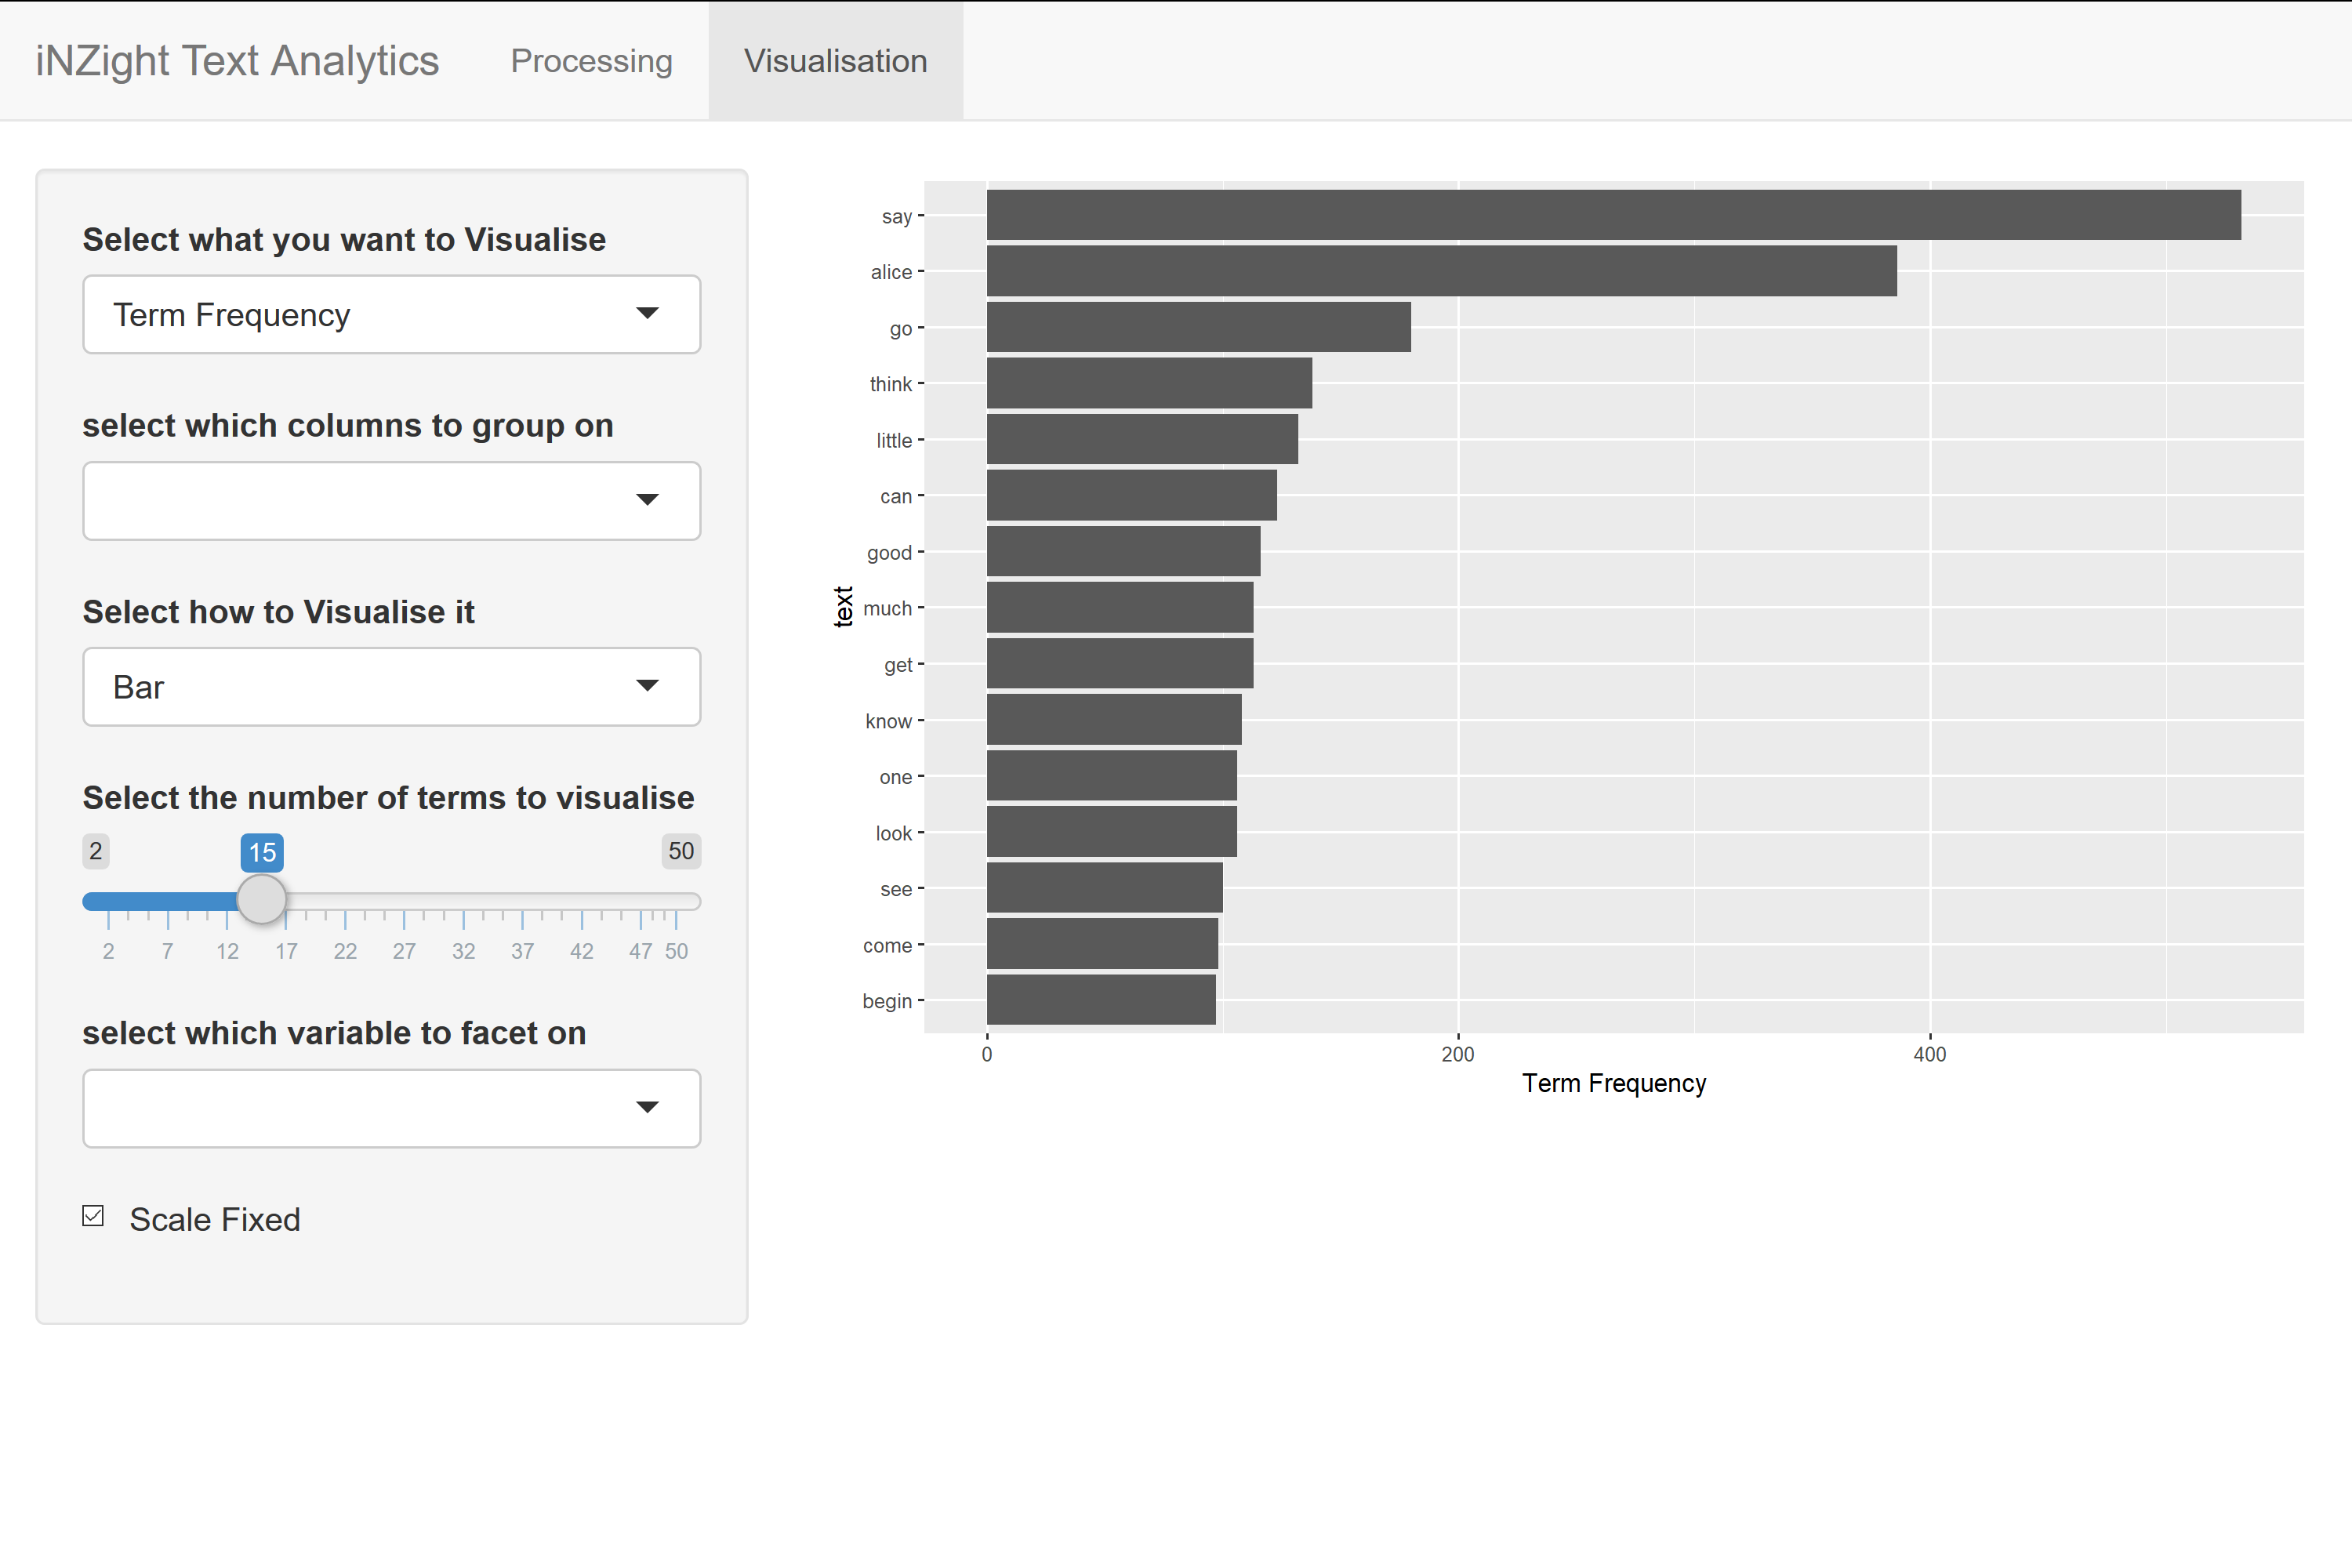
\includegraphics[scale=0.35]{visualisation-overview.png}
  \caption{Visualisation screen\label{fig:visualisation-overview}}
\end{figure}

\begin{figure}
  \centering
  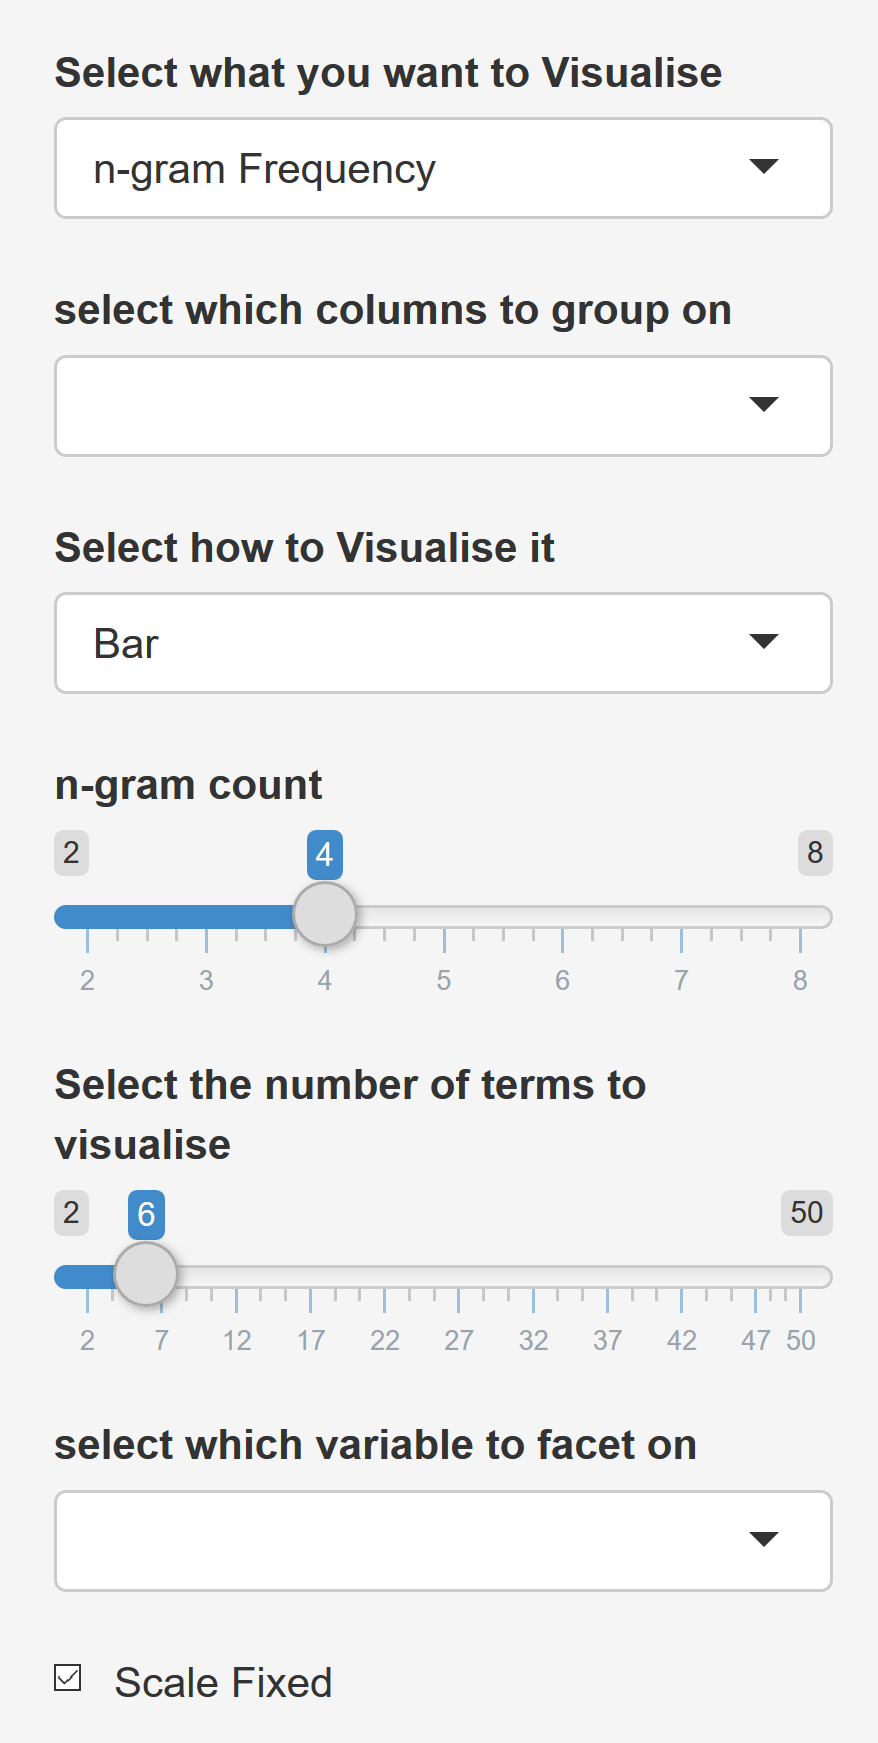
\includegraphics[scale=0.4]{visualisation-n-gram-options.PNG}
  \caption{Options shown when n-gram frequency is
    selected.\label{fig:visualisation-n-gram-options}}
\end{figure}

\subsection{Score}\label{sec:score}

Most insight functions return some numeric measure, typically used as
a score. Visualisations that illustrate the score directly fit into
the ``score'' category. Such visualisations are typically the most
useful in attaining clear analytic results.

\subsubsection{Bar Plot}\label{sec:bar-plot}

Bar plots give the most direct demonstration of scoring for text,
allowing for clear comparisons between terms. A function,
\mintinline{r}{score_barplot()} (\underline{\cref{lst:barplot}}) has
been defined to create bar plots for the data type resulting from the
insight functions. An issue with the implementation of
\mintinline{r}{ggplot2::geom_bar()} is the reliance on factor levels
to provide ordering, which may provide incorrect ordering when
facetting, as factor levels are fixed at a global level for a vector.
\mintinline{r}{tidytext::reorder_within()} purports to solve this
problem, though it has not been used due to the nonsensical coupling
of such a function with the package, and the need to remove
dependencies on the \texttt{tidytext} package.

\subsubsection{Word Cloud}\label{sec:word-cloud}

Word clouds depict a random layout of words of varying sizes
reflecting their scores, and a function named
\mintinline{r}{score_wordcloud()} (\underline{\cref{lst:wordcloud}})
has been created to implement them. They are only about as useful as
pie charts for putting across any more than a rough idea of what the
highest scoring items are. Despite this, they are an oft-requested
form of visualisation, as they really do look good. Building this
functionality in was a guilty pleasure, and the package used to
implement wordclouds, ggwordcloud, is exceedingly well
made\autocite{pennec19}. An in-app example is given in
\underline{\cref{fig:visualisation-keywords-wordcloud}}.

The option is given for a variety of shapes for the word cloud to
take. Future development will allow for a bright range of colours in
the text of the word cloud, to be more aesthetically pleasing.

\begin{figure}
  \centering
  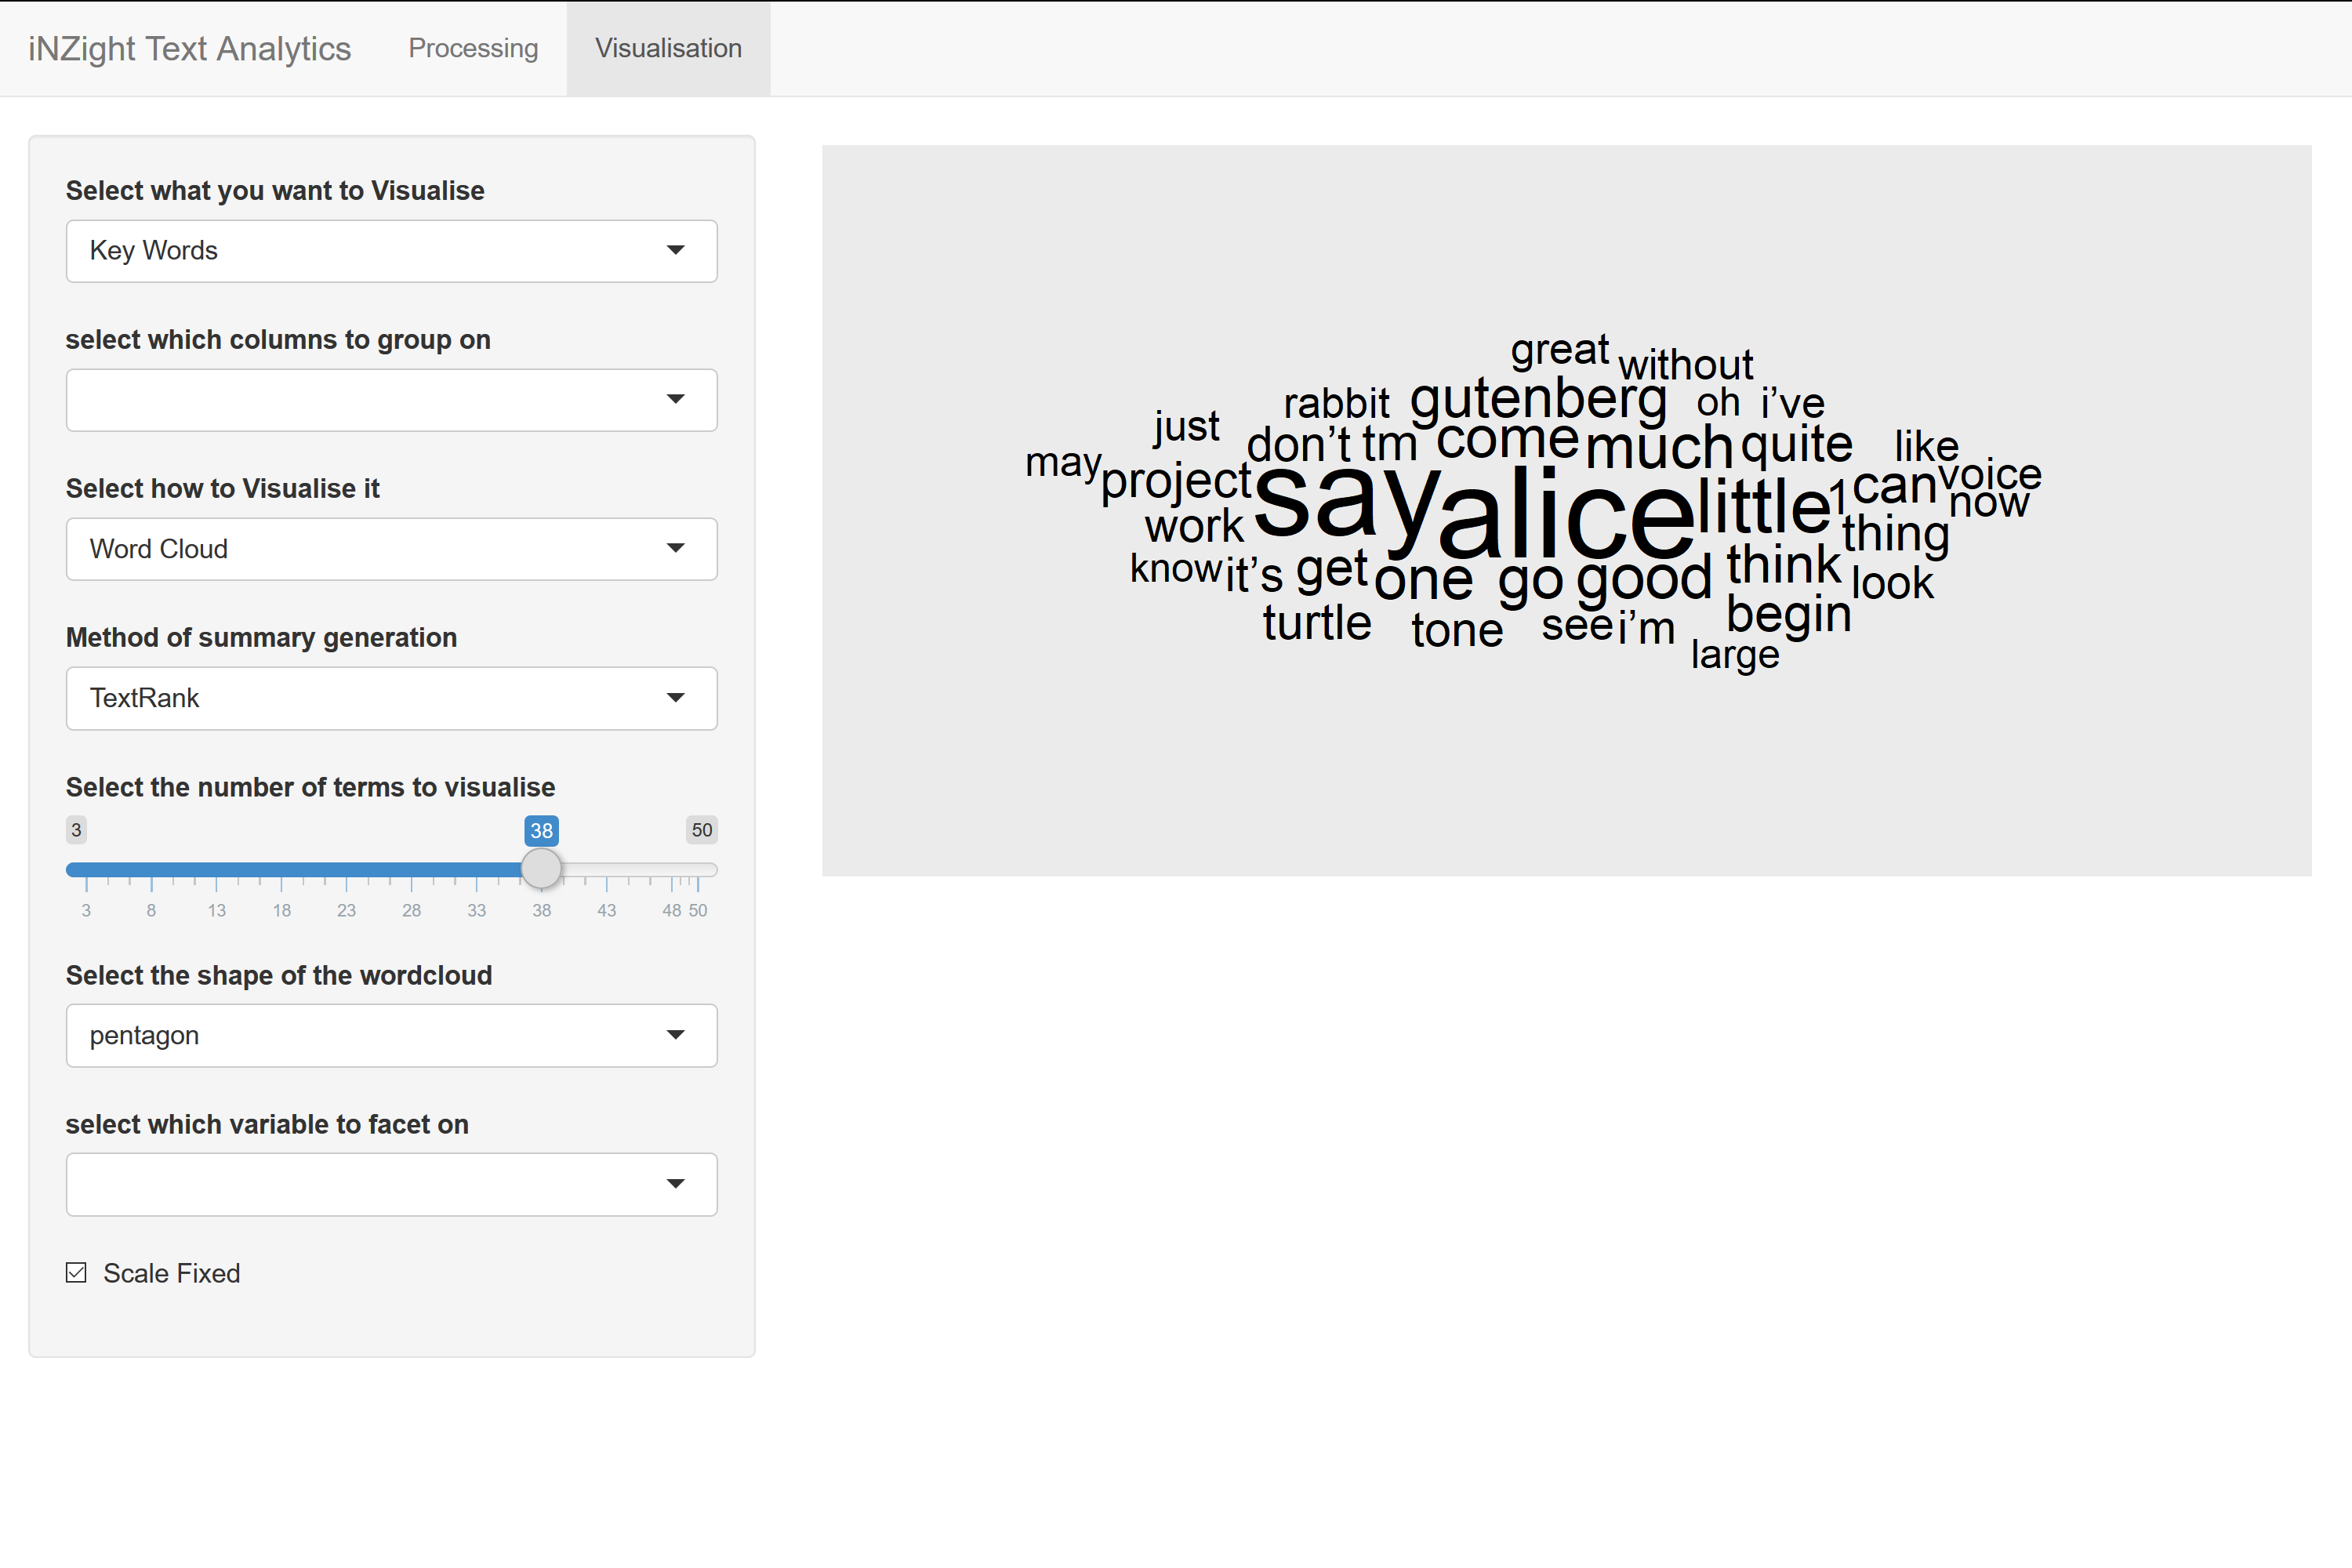
\includegraphics[scale=0.35]{visualisation-keywords-wordcloud.png}
  \caption{Key words visualised with Word
    Cloud\label{fig:visualisation-keywords-wordcloud}}
\end{figure}

\subsection{Distribution}\label{sec:distribution}

The distribution of scores are interesting for their own sake in text
analysis, providing an informative summary of scores over the entirety
of a text. Distributions are particularly enlightening when comparing
between groups, when facetted. Over a large dataset that free-form
survey responses may provide, it is useful to calculate the mean
sentiment for each response, and assess the resulting distribution ---
this program provides such capabilities.

\subsubsection{Histogram}\label{sec:histogram}

Histograms show a discrete distribution of some score. They are
particularly useful for discrete scores, such as the kind produced by
an AFINN sentiment analysis
(\underline{\cref{sec:term-sentiment,fig:visualisation-term-sentiment-hist-facet}}).
A function, \mintinline{r}{dist_hist()} (\cref{lst:histogram}), was
created for visualisation in the form of a histogram.

\begin{figure}
  \centering
  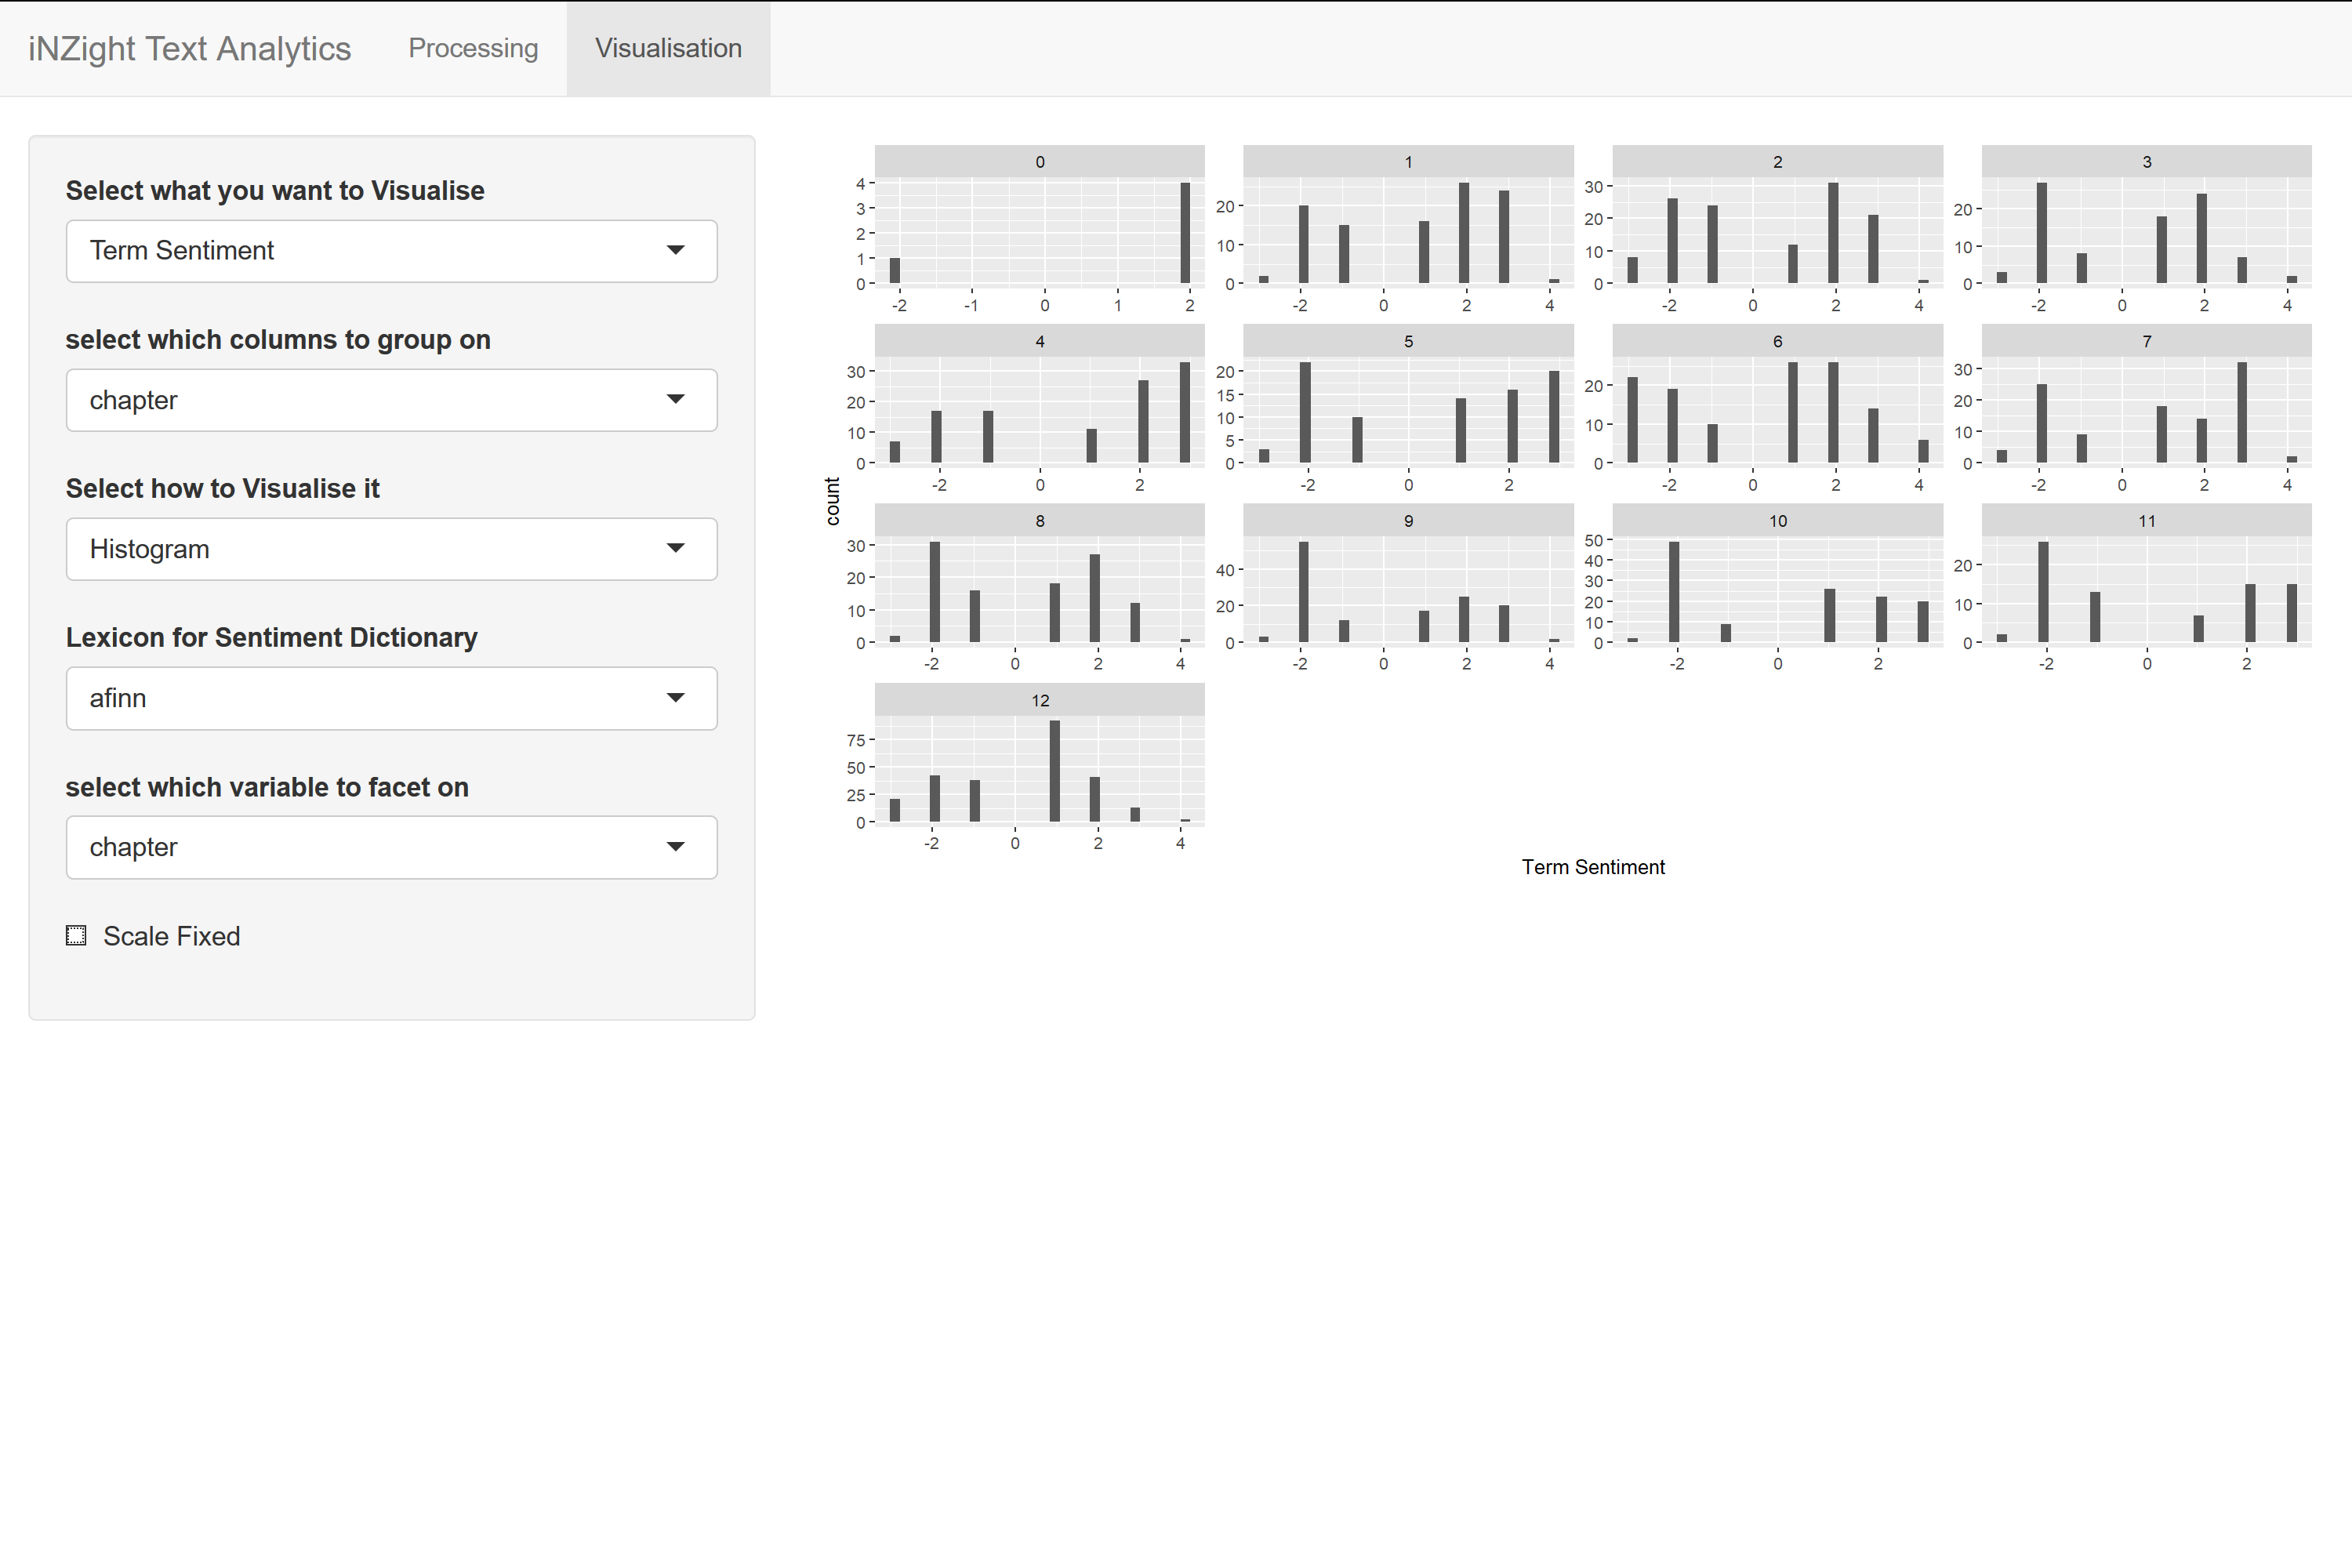
\includegraphics[scale=0.35]{visualisation-term-sentiment-hist-facet.png}
  \caption{Term Sentiment visualised with histograms, facetted by
    chapter\label{fig:visualisation-term-sentiment-hist-facet}}
\end{figure}

\subsubsection{Density}\label{sec:density}

To visualise the density estimation as a continuous distribution for
some score, a function named \mintinline{r}{dist_density()}
(\underline{\cref{lst:density}}) was defined in a similar form to the
histogram visualisation function. Density visualisations work
particularly well for the statistics given by aggregate sentiment
analyses (\underline{\cref{sec:aggregate-sentiment}}). In the
application, they are treated as any other visualisation, just
requiring selection from a drop-down menu, as in
\underline{\cref{fig:visualisation-agg-term-count-density}}.

\begin{figure}
  \centering
  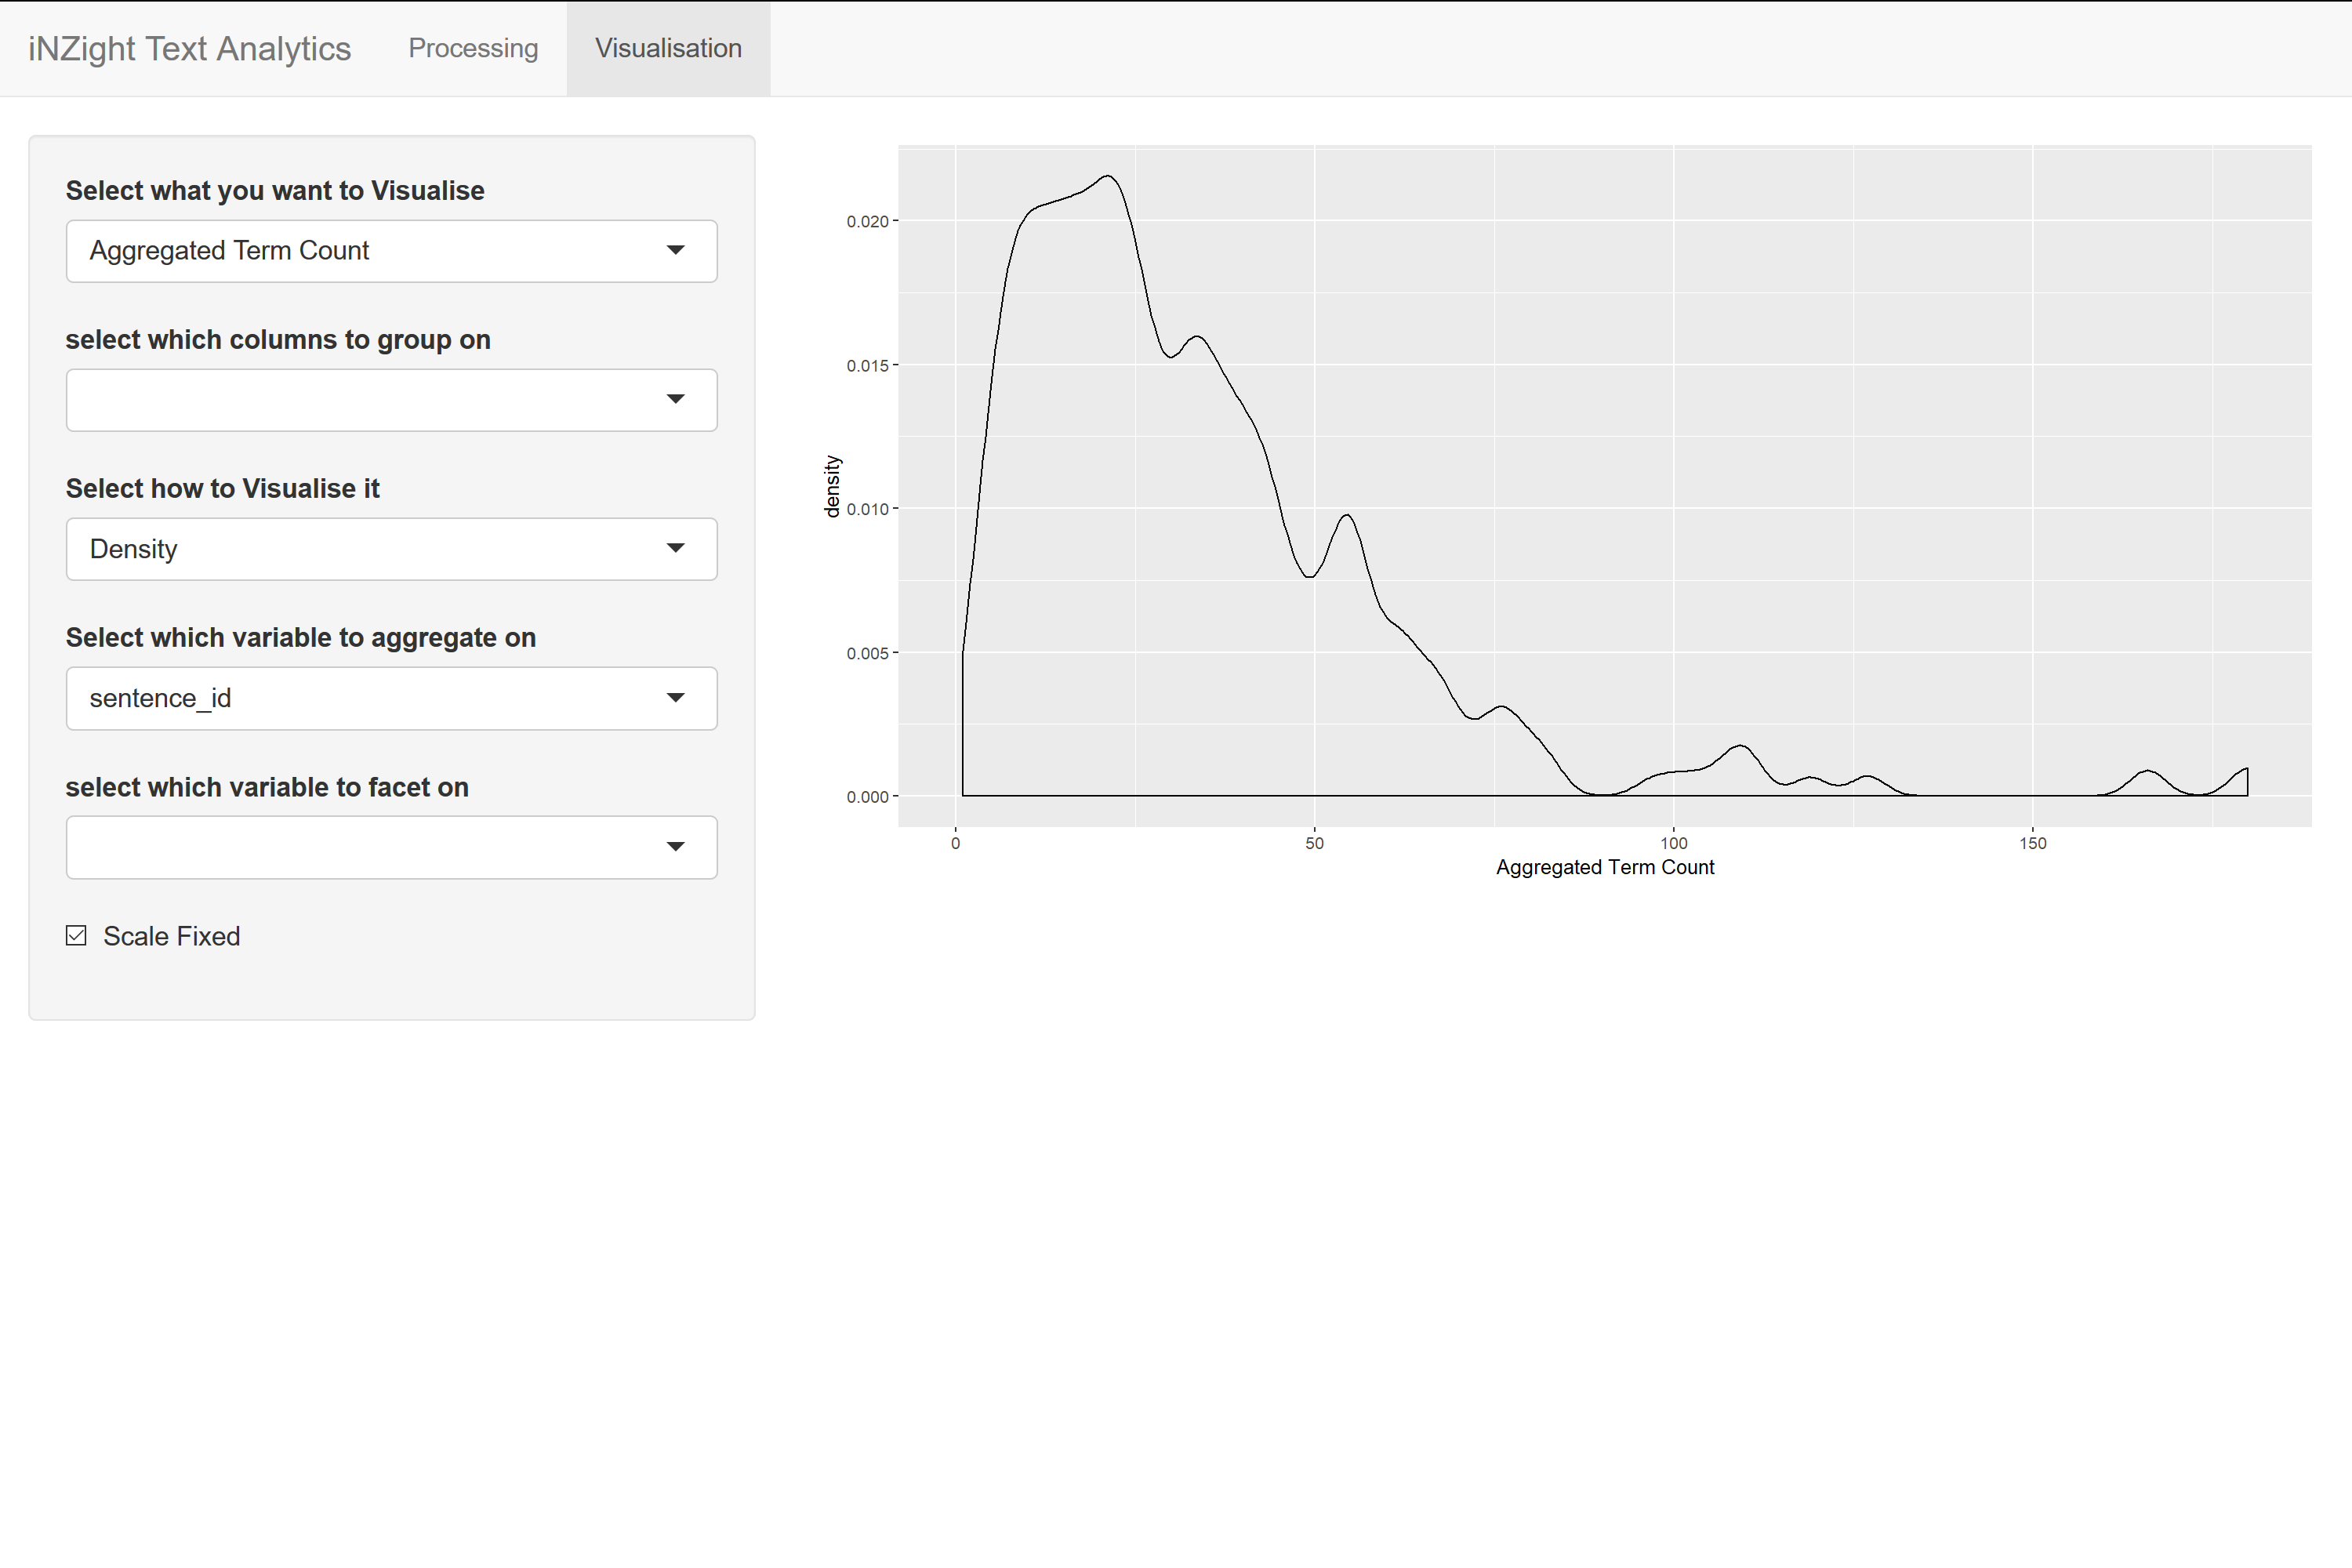
\includegraphics[scale=0.35]{visualisation-agg-term-count-density.png}
  \caption{Aggregate Term Count over sentences visualised as a
    density\label{fig:visualisation-agg-term-count-density}}
\end{figure}

\subsection{Structure}\label{sec:structure}

The structure of the text holds information that no individual piece
of text holds by itself. The evolution of certain characteristics over
time, as well as patterns in the text, can be brought to light with
visualisations of the structure.

\subsubsection{Time Series}\label{sec:time-series}

Treating text as a time series, with each term representing a unit of
time, allows for a running summary of the text from beginning to end.
A function named \mintinline{r}{struct_time_series()}
(\underline{\cref{lst:time-series}}) was composed to capture this form
of visualisation. Time series plots pair particularly well with a
moving-average term-sentiment, as described in
\underline{\cref{sec:moving-average-term}}
(\underline{\cref{lst:ma-term-sentiment}}).

\subsubsection{Page View}\label{sec:page-view}

The concept and function implementation
(\mintinline{r}{struct_pageview()} (\underline{\cref{lst:page-view}})
of page view is based on the visualisation format of the package
\texttt{ggpage}. The intention is for each word in the original text to be
represented as a rectangle on a page, with a width proportional to the
word length. The fill of the rectangle may reflect scores, or even
some category. Future development will have the original text
superimposed over the word placeholders, with the ability to search
through the text. Page view is set as the default for visualising
aggregate and term sentiment in the application
(\underline{\cref{fig:visualisation-agg-sent-pageview}}).

Different colour palettes will also bring clarity to the
visualisation, with only sequential colour palettes being currently
implemented.

The \texttt{R} package \texttt{ggpage} is set up for making immediate
plots, but by using the package's constructor
\mintinline{r}{ggpage_build()} and \mintinline{r}{ggpage_plot()},
complex functions can be formed in the immediate representation from
build before plotting\autocite{hvitfeldt19ggpage}. Facetting is an
issue, with the standard implementation lacking clear support.

Creating this function was the initial impetus for having a lossless
data structure; once stopwords were removed, they were still desired
to be represented in the structure of the text, but with no analytics
performed on them. This was achieved in the program, with stopwords
taking space, but having no coloured fill.

\begin{figure}
  \centering
  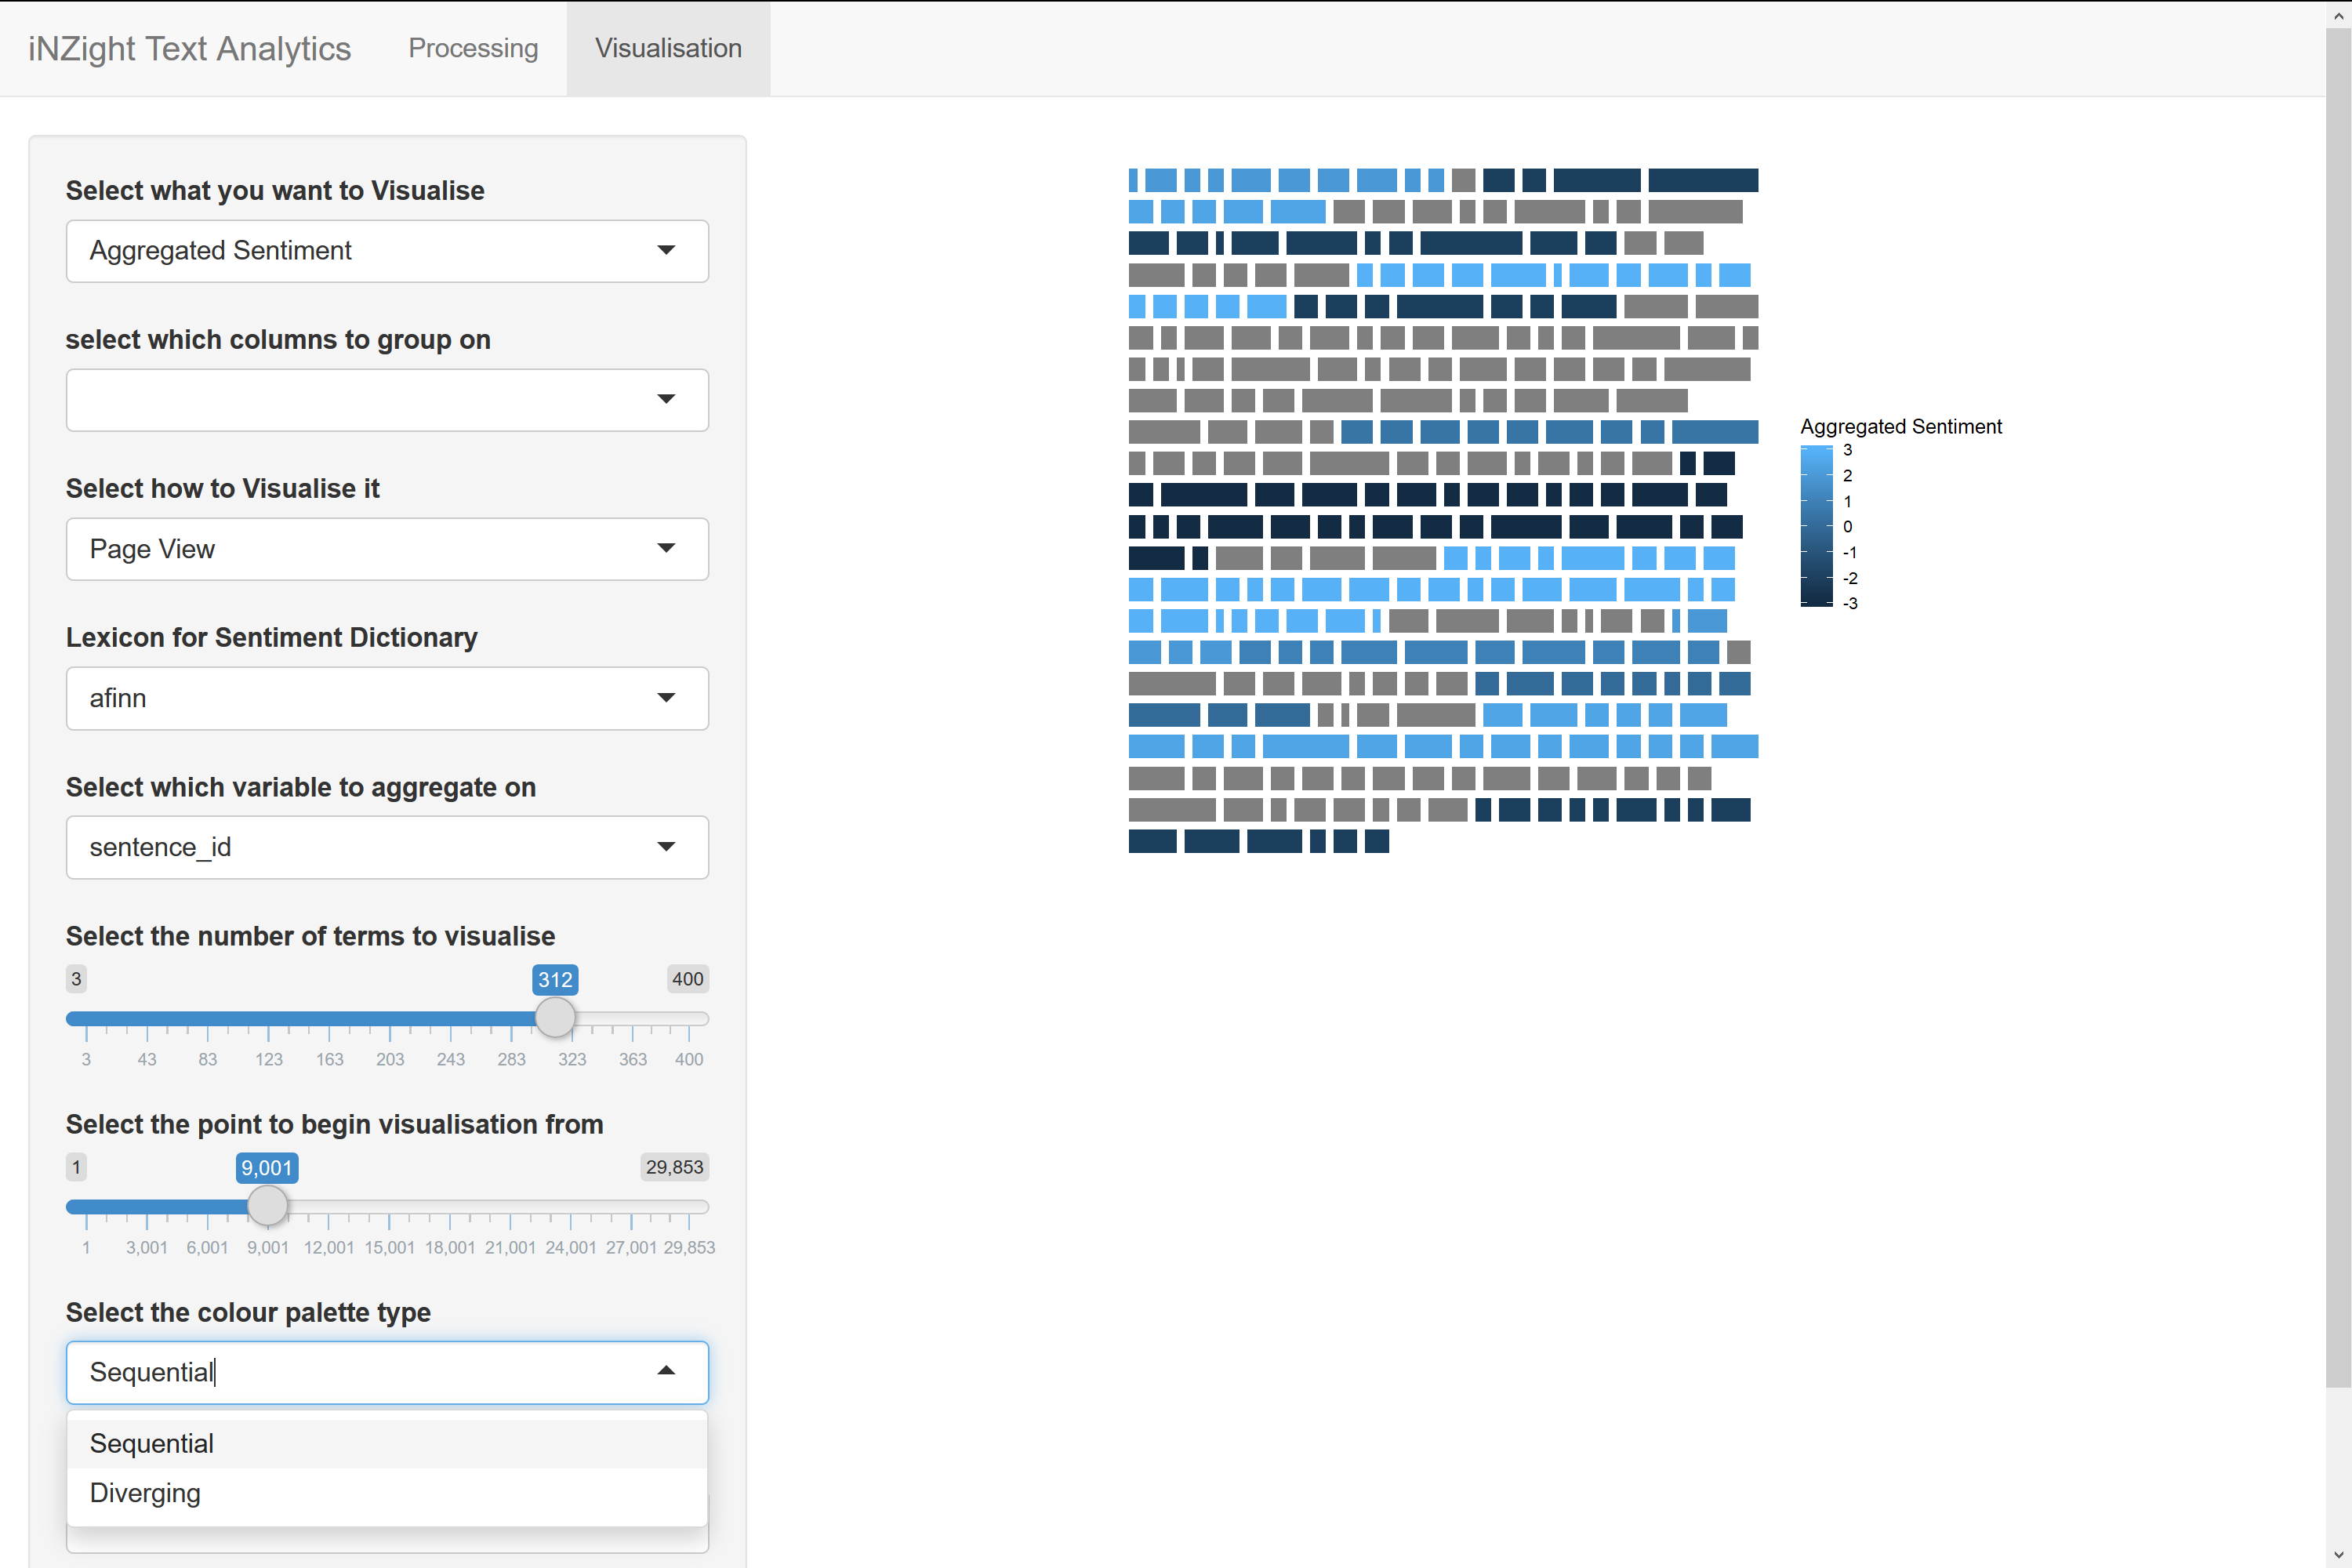
\includegraphics[scale=0.35]{visualisation-agg-sent-pageview.png}
  \caption{Aggregate Sentiment visualised with Page
    View\label{fig:visualisation-agg-sent-pageview}}
\end{figure}

\subsection{Wrapper}\label{sec:wrapper-1}

Visualisation is performed through a wrapper function
\mintinline{r}{get_vis()} (\underline{\cref{lst:get-vis}}), that can
perform the necessary facetting and changes to scaling. The special
case of page view requires additional facetting considerations.

\section{Application}\label{sec:application}

The Shiny web app (\underline{\cref{lst:app}}) is the
frontpiece of the whole program. In about 300 lines of code, it
defines both the interface and the server functions, which call my R
package. As with all shiny applications, it consists of a UI front-end
that is rendered in a web browser for the user to interact with, and a
server back-end that performs the analytic work.

The app consists of two main tabs: processing, and visualisation. The
processing tab is the first screen encountered by a user, allowing
them all of the processing functions offered by the package, in a GUI
interface. Once one or more text files have been imported, lemmatised,
sectioned, etc.\ in the processing tab, the user moves to
visualisation, presented immediately with a default plot from a
default analysis. The user may select a different analysis from a
drop-down list of analyses, which call from the insight functions in
the package, automatically and intelligently. Each analysis has a
default set of options and a visualisation associated with it, so that
as soon as a choice has been made to visualise some text-construct, a
plot instantly appears. Alternative visualisations can be selected
with a drop down menu.

Additional options, for the control of both the analysis and
visualisation, dynamically appear, depending on the type of insight
and associated visualisation. After an insight is selected, the server
generates options related to the insight for the UI, as shown in
\cref{tab:ui-insight-opts}. Similarly, when a visualisation is
selected, the server generates options related to the visualisation
for the UI, as shown in \cref{tab:visopts}.

\begin{landscape}
\begin{table}
  \centering
  \begin{tabular}{llll}
    \toprule
    Insight                       & Insight Options              & Default Options           & Default Visualisation \\
    \midrule
    Term frequency                & ---                          &                           & Bar plot              \\
    n-gram frequency              & n-gram count                 & 2 (bigram)                & Bar plot              \\
    Key words                     & Method of summary generation & TextRank                  & Bar plot              \\
    Term sentiment                & Sentiment lexicon            & AFINN                     & Page view             \\
    Moving average term sentiment & Moving average lag           & 50                        & Time series           \\
                                  & Sentiment lexicon            & AFINN                     &                       \\
    Aggregated term count         & Variable to aggregate on     & Generated from input text & Bar plot              \\
    Key sections                  & Method of summary generation & LexRank                   & Bar plot              \\
                                  & Variable to aggregate on     & Generated from input text &                       \\
    Aggregated sentiment          & Sentiment lexicon            & AFINN                     & Page view             \\
                                  & Variable to aggregate on     & Generated from input text &                       \\
    \bottomrule
  \end{tabular}
  \caption{Dynamically generated UI for insight options\label{tab:ui-insight-opts}}
\end{table}
\end{landscape}


\begin{table} \centering
  \begin{tabular}{lll}
    \toprule
    Visualisation & Visualisation Options                     & Default Options \\
    \midrule
    Word Cloud    & Number of terms to visualise              & 15              \\
                  & Shape of word cloud                       & Circle          \\
    Page Views    & Number of terms to visualise              & 100             \\
                  & Point in text to begin visualisation from & 1               \\
                  & Colour Palette type                       & Sequential      \\
    Bar plot      & Number of terms                           & 15              \\
    Time Series   & ---                                       &                 \\
    Density       & ---                                       &                 \\
    Histogram     & ---                                       &                 \\
    \bottomrule
  \end{tabular}
  \caption{Visualisations and their options\label{tab:visopts}}
\end{table}

All visualisations are additionally affected by the option of facetting
by some variable from the input text.

The application has undergone a rebuild over the course of the
project, starting with an app mirroring the logic of the underlying
text analytics package closely, before moving to a more user-centric
design for interaction.

Originally, the app required a user to perform the preparation stages,
then select what insight functions to perform, before moving on to
visualisation. This was a programmer-centric manner of interaction,
being imperative in the sense that the user had to specify how to
perform the analysis.

This was changed dramatically to be more declarative: The user
performs whatever preparation is necessary, then states what analysis
they want to see, and possibly how they want to see it, and the app
determines what has to happen in the background to deliver on this
request. This is effectively automatic visualisation based on the
insight selection, which is closer to the behaviour and philosophy of
the main iNZight program.

Using a reactive framework in the creation of the app has led to
several difficulties, most notably in the lack of state held by the
central object. To have some capacity for iterative analysis, going
from preparation to visualisation, several successive variables have
been used to pass one logically prior output to the next, with the
final variable being used for the display.

\chapter{Conclusion}\label{cha:conclusion}

\section{Recommendations}\label{sec:recommendations}

\subsection{Future Development}

The next step for this project is to add several additional insight
functions, such as tf-idf scoring, to facilitate ``topic modelling''.
Following this, integration into the main iNZight application can take
place, which won't be as arduous as project integration typically is,
as this program and iNZight both make use of the same Shiny web app
framework.

This project has brought to light many workflows and technologies that
if made use of, would improve the application substantially. As hinted
at in \underline{\cref{sec:why-tidyverse}}, ideally
development would be based around the creation of several carefully
considered classes using R's S4 object oriented system, with a few
basic generic functions for the classes. The functional paradigm has
proved remarkably useful in providing a program that is easy to reason
about, and immutability aids this especially. There is nothing about
this paradigm that precludes the creation of other classes, as Haskell
aptly demonstrates\autocite{Hudak07ahistory}. This move away from a
tidy paradigm would also involve the jettisoning of the residual
dependencies on the \texttt{tidytext} package, and working directly with the
external packages wrapped by \texttt{tidytext} instead.

An object-oriented approach will also allow for further losslessness
in the data. For instance, the behaviour of filtering results in a
subset of the input dataframe, while an object may have methods
defined that simply ``mask'' whatever meets the filtering predicates
--- hiding, instead of deleting, thereby allowing for retrieval later
if needed.

A realistic development that will be easy to implement given some time
is support for in-program access to online text sources such as
Project Gutenberg and Twitter, as forms of general online text
extraction. These would be included as more text import formats are
allowed. In support of the additional text complexity, options for
more complex model-based analyses will be easy to swap in for the
current dictionary-based analyses, using additional arguments to
existing functions that trigger in-function calls to the model-based
analyses. Included in this bundle of work would be more processing
options, including those for existing import formats; for example,
allowing user specification of the text column in a \texttt{csv} file.

Greater user control over components of lexicons would be a worthwhile
pursuit, especially in the specification of stopwords and sentiment.
User-added stopwords and sentiments would provide great utility,
alongside user-specified deletions of words from the base lexicons.
This should be performed in a way that makes it as simple as possible;
tools to aid the user could be a clickable table of common words, to
delete or add to the lexicon.

More visualisation of words in context would be well-received by
users. The ability to search for words and visualise that search in
some form would aid this. A specific implementation of this could make
use of word trees provided by Google Charts, through the
googleVis\autocite{gesmann11} package, which produces network diagrams
of common word orderings (an example depicted in
\underline{\cref{fig:gvis}}). The network diagrams show the common
orderings of words around the searched word, sizing and arranging
according to frequency. Another option is to make use of
``concordance'' tables, which are made heavy use of in corpus
linguistics (\underline{\cref{fig:concordance}}). Concordance tables
find every sentence that the searched word or phrase appears in,
creating a table of these sentences, aligned with the search at the
centre of the table.

\begin{figure}
  \centering 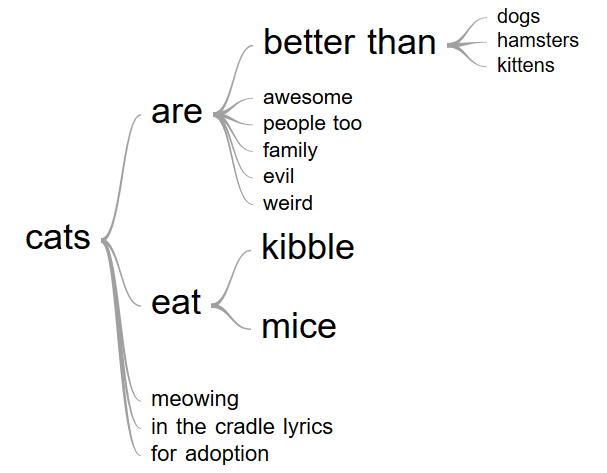
\includegraphics[scale=0.5]{gvis.png}
  \caption{Common word orderings of sentences visualised with word
    trees through the googleVis package\label{fig:gvis}}
\end{figure}

\begin{figure}
  \centering 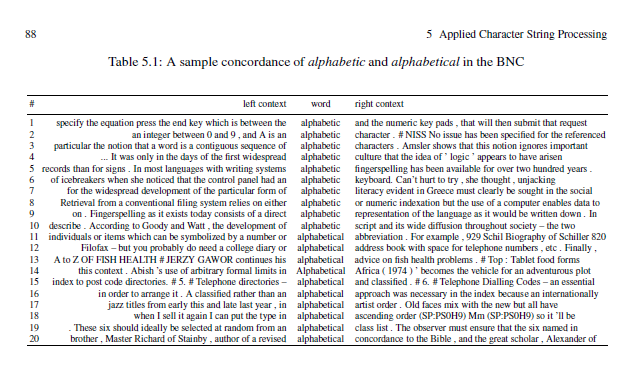
\includegraphics[scale=0.6]{concordance.png}
  \caption{Concordance table of a search for ``alphabetic''\autocite{desagulier17:_corpus_linguis_statis_r}\label{fig:concordance}}
\end{figure}

Another future possibility for development is parallelisation; with
the large size of some text documents, processing time can be
dramatically improved through transforming the text in parallel. The
functional style aids this, as threading is not required to be
consciously determined, as packages exist to transform existing *apply
functions into parallel form.

\subsection{Educational Potential}

The application developed has enormous educational potential for
aiding in learning the basics of text analytics for a very broad range
of students and disciplines. This is primarily due to the structured
approach to text analytics captured in the
preparation-insight-visualisation cycle.

This cycle occurs in a rapid procession in-app, thereby not getting in
the way between learning the theory and seeing the results of an
analysis. The rapid speed of results also allows for experimentation,
which encourages curiosity and reinforces an iterative approach to
analysis.

Finally, while the GUI interface has the natural limitation of
non-scriptability by the end-user, it is far more intuitive for
someone trying to learn text analytics without the cognitive overhead
of having to learn text analytics package API's, the \texttt{R}
language, or concepts of programming in order to perform such
analyses.

\section{Summary}\label{sec:summary}

This project conceptualised and delivered a user-friendly application
with which to perform text analytics, providing powerful processing,
insight, and visualisation functionality. The process of creating the
application led to the development of an \texttt{R} package, serving
as the backend to the applications Shiny GUI.\ The program is intended
to integrate with the existing iNZight application, and should be a
significant educational asset.

\subsection{Closing Remarks}

This project has taught me an enormous amount.

Naturally, I have learnt a great deal about text analytics, a field
that I knew nothing about prior to commencing this project.
Considering text analytics from a statistical perspective has led to
new insights for me in the application of statistical methodology and
procedures.

My programming abilities have improved greatly from seeing through a
highly non-trivial application end-to-end. The added constraint of
following a functional paradigm has challenged me and forced me to
think more creatively in providing solutions. Working with the number
of libraries I have has taught me some (sometimes painful) lessons in
dependency management and version control.

Communication was essential to the success of this project, and I also
learnt a lot about effectively communicating technical information to
people with varying levels of field-specific knowledge.

\appendix
\appendixpage{} \addappheadtotoc{}
\chapter{Listings}\label{cha:appendix}

This appendix chapter includes all of the source code needed to build
the package and application. There are live links in the pdf file
connecting the main discussion to individual listings.

% \begin{listing}[ht]

% framesep=2mm,
% fontsize=\footnotesize,
% linenos
% ]{R}{src/table.R}
% \caption{Example Code}
% \label{lst:test}
% \end{listing}

% \begin{table}[ht]
%   \centering \input{src/output_table}
%   \caption{test table}
%   \label{tab:test}
% \end{table}

\captionof{listing}{Import
  \texttt{txt}\label{lst:import-txt}}\inputminted[frame=lines,fontsize=\scriptsize,xleftmargin=\parindent,linenos]{R}{R/import-txt.R}

\captionof{listing}{Import \texttt{csv}\label{lst:import-csv}}
\inputminted[frame=lines,fontsize=\scriptsize,xleftmargin=\parindent,linenos]{R}{R/import-csv.R}

\captionof{listing}{Import excel\label{lst:import-excel}}
\inputminted[frame=lines,fontsize=\scriptsize,xleftmargin=\parindent,linenos]{R}{R/import-excel.R}

\captionof{listing}{Import files\label{lst:import-files}}
\inputminted[frame=lines,fontsize=\scriptsize,xleftmargin=\parindent,linenos]{R}{R/import-files.R}

\captionof{listing}{Prepare text\label{lst:text-prep}}
\inputminted[frame=lines,fontsize=\scriptsize,xleftmargin=\parindent,linenos]{R}{R/text-prep.R}

\captionof{listing}{Manage stopwords\label{lst:stopwords}}
\inputminted[frame=lines,fontsize=\scriptsize,xleftmargin=\parindent,linenos]{R}{R/stopwords.R}

\captionof{listing}{Format data\label{lst:format-data}}
\inputminted[frame=lines,fontsize=\scriptsize,xleftmargin=\parindent,linenos]{R}{R/format-data.R}

\captionof{listing}{Detect and add sections\label{lst:section}}
\inputminted[frame=lines,fontsize=\scriptsize,xleftmargin=\parindent,linenos]{R}{R/section.R}

\captionof{listing}{Determine Term Frequencies\label{lst:term-freq}}
\inputminted[frame=lines,fontsize=\scriptsize,xleftmargin=\parindent,linenos]{R}{R/term-freq.R}

\captionof{listing}{Get n-grams\label{lst:get-ngram}}
\inputminted[frame=lines,fontsize=\scriptsize,xleftmargin=\parindent,linenos]{R}{R/get-ngram.R}

\captionof{listing}{Get n-grams frequencies\label{lst:get-ngram-freq}}
\inputminted[frame=lines,fontsize=\scriptsize,xleftmargin=\parindent,linenos]{R}{R/ngram-freq.R}

\captionof{listing}{Determine Key Words with Textrank\label{lst:keywords}}
\inputminted[frame=lines,fontsize=\scriptsize,xleftmargin=\parindent,linenos]{R}{R/keywords.R}

\captionof{listing}{Determine Term Sentiments\label{lst:term-sentiment}}
\inputminted[frame=lines,fontsize=\scriptsize,xleftmargin=\parindent,linenos]{R}{R/term-sentiment.R}

\captionof{listing}{Determine the Moving Average Term Sentiment\label{lst:ma-term-sentiment}}
\inputminted[frame=lines,fontsize=\scriptsize,xleftmargin=\parindent,linenos]{R}{R/ma-term-sentiment.R}

\captionof{listing}{Determine the term count over some aggregate\label{lst:term-count}}
\inputminted[frame=lines,fontsize=\scriptsize,xleftmargin=\parindent,linenos]{R}{R/term-count.R}

\captionof{listing}{Determine the Key Sections\label{lst:key-sections}}
\inputminted[frame=lines,fontsize=\scriptsize,xleftmargin=\parindent,linenos]{R}{R/key-aggregates.R}

\captionof{listing}{Determine the Aggregate Sentiments\label{lst:aggregate-sentiment}}
\inputminted[frame=lines,fontsize=\scriptsize,xleftmargin=\parindent,linenos]{R}{R/aggregate-sentiment.R}

\captionof{listing}{Insight functions wrapper\label{lst:get-insight}}
\inputminted[frame=lines,fontsize=\scriptsize,xleftmargin=\parindent,linenos]{R}{R/get-insight.R}

\captionof{listing}{Bind aggregate terms\label{lst:bind-aggregate}}
\inputminted[frame=lines,fontsize=\scriptsize,xleftmargin=\parindent,linenos]{R}{R/insight-aggregate.R}

\captionof{listing}{Create Bar Plot\label{lst:barplot}}
\inputminted[frame=lines,fontsize=\scriptsize,xleftmargin=\parindent,linenos]{R}{R/barplot.R}

\captionof{listing}{Create Word Cloud\label{lst:wordcloud}}
\inputminted[frame=lines,fontsize=\scriptsize,xleftmargin=\parindent,linenos]{R}{R/wordcloud.R}

\captionof{listing}{Create Histogram\label{lst:histogram}}
\inputminted[frame=lines,fontsize=\scriptsize,xleftmargin=\parindent,linenos]{R}{R/histogram.R}

\captionof{listing}{Create Kernel Density Estimate Plot\label{lst:density}}
\inputminted[frame=lines,fontsize=\scriptsize,xleftmargin=\parindent,linenos]{R}{R/density.R}

\captionof{listing}{Create Time Series Plot\label{lst:time-series}}
\inputminted[frame=lines,fontsize=\scriptsize,xleftmargin=\parindent,linenos]{R}{R/time-series.R}

\captionof{listing}{Create Page View Plot\label{lst:page-view}}
\inputminted[frame=lines,fontsize=\scriptsize,xleftmargin=\parindent,linenos]{R}{R/page-view.R}

\captionof{listing}{Create Visualisation\label{lst:get-vis}}
\inputminted[frame=lines,fontsize=\scriptsize,xleftmargin=\parindent,linenos]{R}{R/get-vis.R}

\captionof{listing}{UI and Server of Shiny Application\label{lst:app}}
\inputminted[frame=lines,fontsize=\scriptsize,xleftmargin=\parindent,linenos]{R}{R/app.R}

\chapter{Package Manual}\label{cha:package-manual}
This appendix chapter consists of a copy of the documentation for the
\texttt{R} package, which was automatically generated through the
Roxygen2 system from in-source comments.

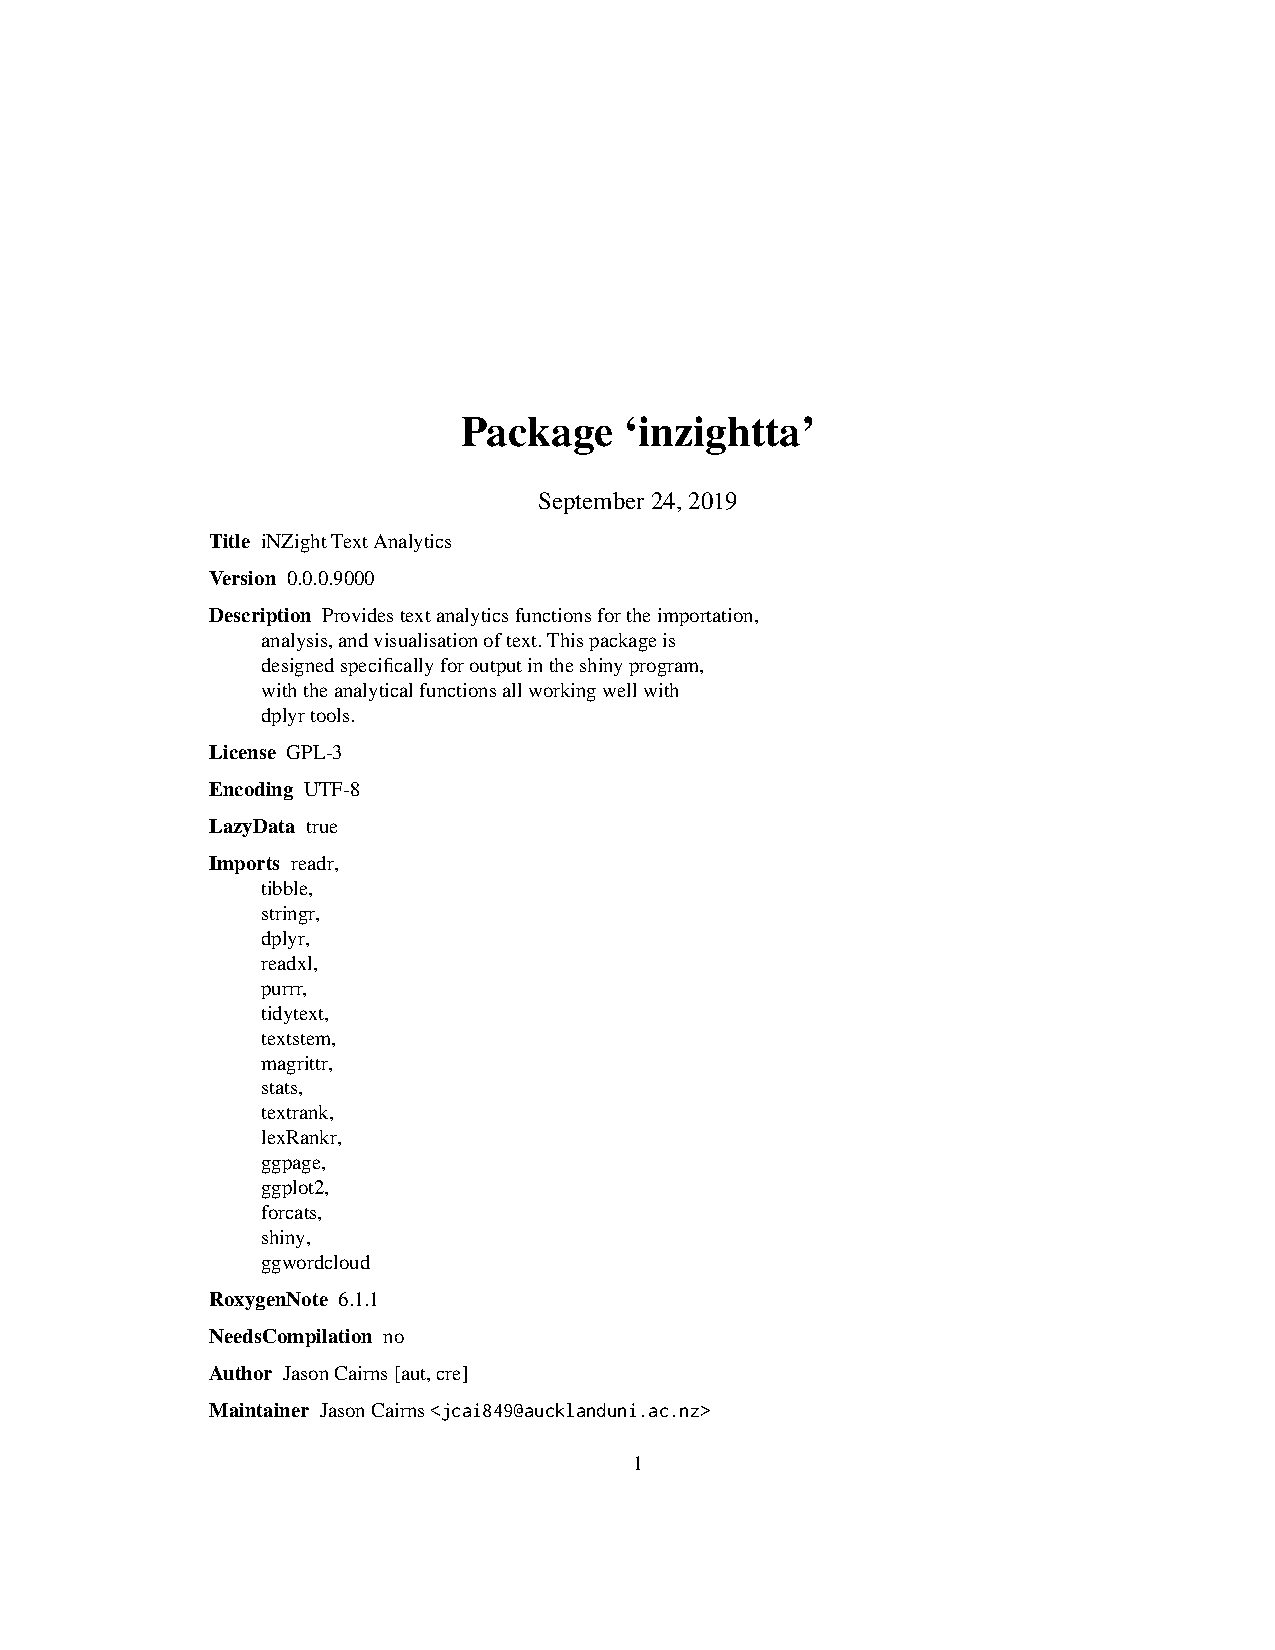
\includepdf[pages=-]{inzightta_manual.pdf}

% \backmatter
\addcontentsline{toc}{chapter}{Glossary} \printglossaries{}
\addcontentsline{toc}{chapter}{Bibliography} \printbibliography{}
\end{document}
